\documentclass[titlepage, a4paper, reqno, openany]{report}
%%%%%%%%%%%%%%%%%%%%%%%%%%%%%%%%%%%%%%%%%%%%%%%%%%%%%%%%%%%%%%%%%%%%%
%%%%%%%%%%%%%%%%%%%%%%%%%%%%%%%%%%%%%%%%%%%%%%%%%%%%%%%%%%
%%			PREAMBLE LATEX GENERAL USE
%%	author: sergio manuel salazar dos santos
%%	email: sergio.salazar.santos@gmail.com
%%	Comment:
%%		Stable, no issues found yet.
%%		Note sequence is importante, and beware of clatching packages.
%%
%%		review: 24032023
%%
%%%%%%%%%%%%%%%%%%%%%%%%%%%%%%%%%%%%%%%%%%%%%%%%%%%%%%%%%%
% preloaded:
% longtable, xcolor, graphicx, booktabs, caption, csquotes, hyperref,
% calc, listings, datetime2, siunitx, geometry, enumitem
%%%%%%%%%%%%%%%%%%%%%%%%%%%%%%%%%%%%%%%%%%%%%%%%%%%%%%%%%%
\usepackage[utf8]{inputenc}
\usepackage[T1]{fontenc}
\usepackage{lmodern}
\usepackage[portuguese]{babel}
%%%%%%%%%%%%%%%%%%%%%%%%%%%%%%%%%%%%%%%%%%%%%%%%%%%%%%%%%%
\usepackage{scrbase} % Required for handling language-dependent names of sections/document elements
\usepackage{scrhack} % Loads fixes for various packages
\usepackage{longtable} % Required for tables that span multiple pages 
\usepackage[dvipsnames, svgnames, table]{xcolor} % Required for specifying custom colours
\usepackage{graphics}
\usepackage{booktabs}
\usepackage[autostyle=true]{csquotes}
\usepackage{calc}
\usepackage{listings}
\RequirePackage[calc,portuguese]{datetime2}	% For date format
%\usepackage[calc, en-US]{datetime2}
\usepackage{siunitx}
\usepackage{paralist}
\usepackage{makeidx}
\usepackage{titlepic}
\usepackage{ragged2e}
\usepackage{blindtext}
\usepackage{hyphsubst}
\usepackage[top=2cm,left=1.5cm,right=1.2cm,bottom=2cm]{geometry}
\usepackage{graphicx}
\usepackage[graphicx]{realboxes}
\usepackage{hyphenat}
\usepackage{color,colortbl}
\usepackage[dvipsnames, svgnames, table]{xcolor}
%%%%%%%%%%%%%FIXED ORDER%%%%%%%%%FIXED ORDER%%%%%%%%%%%%%%
%\usepackage[shortcuts, nopostdot, acronym, toc, nogroupskip, nonumberlist, automake]{glossaries}
\usepackage[acronym, toc, shortcuts, acronymlists={hidden}, nopostdot, nogroupskip, nonumberlist, automake=immediate]{glossaries} %for lists of terms, acronyms and symbols
%\usepackage[nottoc]{tocbibind}
%%%%%%%%%%%%%%%%%%%%%%%%%%%%%%%%%%%%%%%%%%%%%%%%%%%%%%%%%%
%%%%%%%%%%%%%%%%%%%%%%%%%%%%%%%%%%%%%%%%%%%%%%%%%%%%%%%%%%
% FYI, the following packages are preloaded with the document class:
% longtable, xcolor, graphicx, booktabs, caption, csquotes, hyperref,
% calc, listings, datetime2, siunitx, geometry, enumitem
%%%%%%%%%%%%%%%%%%% extra packages %%%%%%%%%%%%%%%%%%%%%%%
\usepackage{amsmath}		% the principal package in the AMS-LATEX distribution
\usepackage{amsfonts}		% extended set of fonts for use in mathematics
\usepackage{amssymb}		% adds new symbols to be used in math mode
\usepackage{mathrsfs}		% math fonts, e.g., Laplace
\usepackage{float}			% provides the H float modifier option
\usepackage{multirow}		% tables \multirow command
\usepackage{subcaption}		% enables subfigures
\usepackage{lscape}			% for landscape mode
\usepackage{verbatim}		% new verbatim environment, \begin{comment}...\end{comment}, \verbatiminput
%%%%%%%%%%%%%%%%%%%%%%%%%%%%%%%%%%%%%%%%%%%%%%%%%%%%%%%%%%
%add extra packages if needed here
%%%%%%%%%%%%%%%%%%%%%%%%%%%%%%%%%%%%%%%%%%%%%%%%%%%%%%%%%%
\usepackage{etoolbox}
\usepackage{xparse}
\usepackage[font=small, labelfont=bf]{caption}
\usepackage{hyphenat}
\usepackage{multicol}
\usepackage{makecell}
\usepackage{array}
\usepackage{tabularx}
\usepackage[export]{adjustbox}
\usepackage{eurosym}
\usepackage{enumitem} %% conflict never put enumitem with enumerate
%\usepackage{enumerate} %% conflict never put enumitem with enumerate
\usepackage{longtable}
\usepackage{setspace}
\usepackage{lipsum}
\usepackage{moreverb}
\usepackage{rotating}
\usepackage{romannum}
%%%%%%%%%%%%%%%%%%%%%%%%%%%%%%%%%%%%%%%%%%%%%%%%%%%%%%%%%%
\usepackage[portuguese]{babelbib}
\usepackage[toc, page]{appendix}
%%%%%%%%%%%%%%%%%%%%%%%%%%%%%%%%%%%%%%%%%%%%%%%%%%%%%%%%%%
\usepackage{url}
\usepackage[hidelinks]{hyperref}
\usepackage[hyperpageref]{backref}
%%%%%%%%%%%%%%%%%%%%%%%%%%%%%%%%%%%%%%%%%%%%%%%%%%%%%%%%%%
\usepackage{pgfgantt}
\usepackage{tikz}
\usepackage{circuitikz}
%%%%%%%%%%%%%%%%%%%%%%%%%%%%%%%%%%%%%%%%%%%%%%%%%%%%%%%%%%
\usepackage[tickmarkheight=5em,textwidth=\marginparwidth,textsize=small]{todonotes} % insert small notes [\todo[inline]{<message>} and \listoftodos]
%%%%%%%%%%%%%%%%%%%%%%%%%%%%%%%%%%%%%%%%%%%%%%%%%%%%%%%%%%
%%%%%%%%%%%%%%%%%%%%%%%%%%%%%%%%%%%%%%%%%%%%%%%%%%%%%%%%%%%%%%%%
\usetikzlibrary{matrix, shapes.geometric, arrows, trees, positioning, calc}
\graphicspath{{image/}{image/logo/}{figure/}}
%\selectbiblanguage{portuguese}
%\setbtxfallbacklanguage{english}
%%%%%%%%%%%%%%%%%%%%%%%%%%%%%%%%%%%%%%%%%%%%%%%%%%%%%%%%%%%%%%%%
\bibliographystyle{babplain}
%\bibliographystyle{plain}
%\bibliographystyle{ieeetr}
%%%%%%%%%%%%%%%%%%%%%%%%%%%%%%%%%%%%%%%%%%%%%%%%%%%%%%%%%%%%%%%%
%%%%%%%%%%%%%%%%%%%%%%%%%%%%%%%%%%%%%%%%%%%%%%%%%%%%%%%%%%
\usepackage[markcase=used]{scrlayer-scrpage}
%%%%%%%%%%%%%%%%%%%%%%%%%%%%%%%%%%%%%%%%%%%%%%%%%%%%%%%%%%%%%%%%
\usetikzlibrary{matrix, shapes.geometric, arrows, trees, positioning, calc}
\graphicspath{{image/}{image/logo/}{figure/}}
%%%%%%%%%%%%%%%%%%%%%%%%%%%%%%%%%%%%%%%%%%%%%%%%%%%%%%%%%%%%%%%%
\bibliographystyle{babplain}
%\bibliographystyle{plain}
%\bibliographystyle{ieeetr}
%%%%%%%%%%%%%%%%%%%%%%%%%%%%%%%%%%%%%%%%%%%%%%%%%%%%%%%%%%%%%%%%

%%%%%%%%%%%%%%%%%%%%%%%%%%%%%%%%%%%%%%%%%%%%%%%%%%%%%%%%%%
% FYI, the following packages are preloaded with the document class:
% longtable, xcolor, graphicx, booktabs, caption, csquotes, hyperref,
% calc, listings, datetime2, siunitx, geometry, enumitem
%%%%%%%%%%%%%%%%%%% extra packages %%%%%%%%%%%%%%%%%%%%%%%
\usepackage{amsmath}		% the principal package in the AMS-LATEX distribution
\usepackage{amsfonts}		% extended set of fonts for use in mathematics
\usepackage{amssymb}		% adds new symbols to be used in math mode
\usepackage{mathrsfs}		% math fonts, e.g., Laplace
\usepackage{float}			% provides the H float modifier option
\usepackage{multirow}		% tables \multirow command
\usepackage{subcaption}		% enables subfigures
\usepackage{lscape}			% for landscape mode
\usepackage{verbatim}		% new verbatim environment, \begin{comment}...\end{comment}, \verbatiminput
%%%%%%%%%%%%%%%%%%%%%%%%%%%%%%%%%%%%%%%%%%%%%%%%%%%%%%%%%%
%add extra packages if needed here
%%%%%%%%%%%%%%%%%%%%%%%%%%%%%%%%%%%%%%%%%%%%%%%%%%%%%%%%%%
\usepackage{etoolbox}
\usepackage{xparse}
\usepackage[font=small, labelfont=bf]{caption}
\usepackage{hyphenat}
\usepackage{multicol}
\usepackage{makecell}
\usepackage{array}
\usepackage{tabularx}
\usepackage[export]{adjustbox}
\usepackage{eurosym}
\usepackage{enumitem} %% conflict never put enumitem with enumerate
%\usepackage{enumerate} %% conflict never put enumitem with enumerate
\usepackage{longtable}
\usepackage{setspace}
\usepackage{lipsum}
\usepackage{moreverb}
\usepackage{rotating}
\usepackage{romannum}
%%%%%%%%%%%%%%%%%%%%%%%%%%%%%%%%%%%%%%%%%%%%%%%%%%%%%%%%%%
\usepackage[portuguese]{babelbib}
\usepackage[toc, page]{appendix}
%%%%%%%%%%%%%%%%%%%%%%%%%%%%%%%%%%%%%%%%%%%%%%%%%%%%%%%%%%
\usepackage{url}
\usepackage[hidelinks]{hyperref}
\usepackage[hyperpageref]{backref}
%%%%%%%%%%%%%%%%%%%%%%%%%%%%%%%%%%%%%%%%%%%%%%%%%%%%%%%%%%
\usepackage{pgfgantt}
\usepackage{tikz}
\usepackage{circuitikz}
%%%%%%%%%%%%%%%%%%%%%%%%%%%%%%%%%%%%%%%%%%%%%%%%%%%%%%%%%%
\usepackage[tickmarkheight=5em,textwidth=\marginparwidth,textsize=small]{todonotes} % insert small notes [\todo[inline]{<message>} and \listoftodos]
%%%%%%%%%%%%%%%%%%%%%%%%%%%%%%%%%%%%%%%%%%%%%%%%%%%%%%%%%%
%%%%%%%%%%%%%%%%%%%%%%%%%%%%%%%%%%%%%%%%%%%%%%%%%%%%%%%%%%%%%%%%
\usetikzlibrary{matrix, shapes.geometric, arrows, trees, positioning, calc}
\graphicspath{{image/}{image/logo/}{figure/}}
%\selectbiblanguage{portuguese}
%\setbtxfallbacklanguage{english}
%%%%%%%%%%%%%%%%%%%%%%%%%%%%%%%%%%%%%%%%%%%%%%%%%%%%%%%%%%%%%%%%
\bibliographystyle{babplain}
%\bibliographystyle{plain}
%\bibliographystyle{ieeetr}
%%%%%%%%%%%%%%%%%%%%%%%%%%%%%%%%%%%%%%%%%%%%%%%%%%%%%%%%%%%%%%%%
%%%%%%%%%%%%%%%%%%%%%%%%%%%%%%%%%%%%%%%%%%%%%%%%%%%%%%%%%%%%%%%%%%%%%%%
							%%%SPACING%%%
%%%%%%%%%%%%%%%%%%%%%%%%%%%%%%%%%%%%%%%%%%%%%%%%%%%%%%%%%%%%%%%%%%%%%%%
\newcommand{\minipagespace}[1]{\hfill  \vspace{#1} \newline}
\newcommand{\emptyline}{\hfill \vspace{\baselineskip} \newline}
\newcommand{\emptyspace}[1]{\hfill \vspace{#1} \newline}
\newcommand{\tablespace}[1]{\hfill \vspace{#1} \newline}
\newcommand{\figurespace}[1]{\hfill \vspace{#1} \newline}
\newcommand{\graphicspace}[1]{\hfill \vspace{#1} \newline}
\newcommand{\listingspace}[1]{\hfill \vspace{#1} \newline}
\newcommand{\equationspace}[1]{\hfill \vspace{#1} \newline}
%%%%%%%%%%%%%FIX SECTION NUMBERING IN CASE REPORT%%%%%%%%%%%%%%%%%%%%%%
%\renewcommand\thesection{\arabic{section}}
%\renewcommand\thesubsection{\thesection.\arabic{subsection}}
%\renewcommand\thesubsubsection{\thesection.\thesubsection.\arabic{subsubsection}}
%%%%%%%%%%%%%%%%%%%%%%%%%%%%%%%%%%%%%%%%%%%%%%%%%%%%%%%%%%%%%%%%%%%%%%%
\newcolumntype{L}[1]{>{\raggedright\arraybackslash}p{#1}}
\newcolumntype{C}[1]{>{\centering\arraybackslash}p{#1}}
\newcolumntype{R}[1]{>{\raggedleft\arraybackslash}p{#1}}
%%%%%%%%%%%%%%%%%%%%%%%%%%%%%%%%%%%%%%%%%%%%%%%%%%%%%%%%%%%%%%%%%%%%%%%
\newcommand\acrfullr[2][]{\acrshort[#1]{#2} (\acrlong[#1]{#2})}
%%%%%%%%%%%%%%%%%%%%%%%%%%%%%%%%%%%%%%%%%%%%%%%%%%%%%%%%%%%%%%%%%%%%%%%
\def\mcirc{\mathbin{\scalerel*{\bigcirc}{t}}}
\def\msquare{\mathord{\scalerel*{\Box}{gX}}}
\def\ce{\mathrm{e}}
%%%%%%%%%%%%%%%%%%%%%%%%%%%%%%%%%%%%%%%%%%%%%%%%%%%%%%%%%%%%%%%%%%%%%%%
%\date{\rule[180pt]{0pt}{5pt}}
%%%%%%%%%%%FIX SECTION NUMBERING IN CASE REPORT%%%%%%%%%%%%%%%%%%%%%%%%
\renewcommand\thesection{\arabic{section}}
\renewcommand\thesubsection{\thesection.\arabic{subsection}}
\renewcommand\thesubsubsection{\thesection.\thesubsection.\arabic{subsubsection}}
%%%%%%%%%%%%%%%%%%%%%%%%%%%%%%%%%%%%%%%%%%%%%%%%%%%%%%%%%%%%%%%%%%%%%
\begin{titlepage}
	\title{
		
\includegraphics[scale=0.60]{./image/capa/ISEP_marca_cor_grande.png}
		\emptyline
		\begin{center}
		 	Comportamento Organizacional
		\end{center}		
	}
	\author{
		\begin{minipage}{1\linewidth}
			\begin{minipage}{0.4\linewidth}
				\flushleft
				\textbf{Aluno} : \\
				\emph{S\'{e}rgio Santos},\;$N^o$:\; 1020881 \\
				%\emph{Nome 2},\;$N^o$:\; 2000000\\
				%\emph{Nome 3},\;$N^o$:\; 3000000\\
				%\emph{Nome 4},\;$N^o$:\; 4000000\\
				%\emph{Nome 5},\;$N^o$:\; 5000000\\
			\end{minipage}
			\hspace{0.1\linewidth}
			\fbox{
				\begin{minipage}{0.4\linewidth}
					\centering
					\textbf{Docente/Orientador} \\
					Maria Raposo, \textit{mrp} \\
					\textbf{Unidade Curricular} \\
					CORGA \\
				\end{minipage}
			}
		\end{minipage}
		\minipagespace{2cm}
	}
	\date{Junho 2021} %% enable to hide date
	\titlepic{
		\begin{flushleft}
			\graphicspace{4cm}
			
\includegraphics[scale=0.50]{./image/ROQ/ROQ.jpg}
		\end{flushleft}
	}
\end{titlepage}
%%%%%%%%%%%%%%%%%%%%%%%%%%%%%%%%%%%%%%%%%%%%%%%%%%%%%%%%%%%%%%%%%%%%
%%%%%%%%%%%%%%%%%%%%%%%%%%%%%%%%%%%%%%%%%%%%%%%%%%%%%%%%%%%%%%%%%%%%
%%%%%%%%%%%%%%%%%%%%%%%%%%%%%%%%%%%%%%%%%%%%%%%%%%%%%%%%%%%%%%%%
						%%%GLOSSARY%%%
%%%%%%%%%%%%%%%%%%%%%%%%%%%%%%%%%%%%%%%%%%%%%%%%%%%%%%%%%%%%%%%%
\newglossaryentry{gloss}{
	name={glossário}, 
	description={é uma lista alfabética de termos de um determinado domínio de conhecimento com a definição desses mesmos termos.},
}

\newglossaryentry{pack}{
	name={\textit{package}}, 
	description={é um ficheiro ou conjunto de ficheiros que contêm comandos \LaTeX{} extra que adicionam novas funcionalidades de estilo ou modificam aquelas já existentes.},
	sort={package}	%needed for sorting when using LaTeX commands in the 'name' field
}

\newglossaryentry{lipsum}{
	name={\textit{Lorem Ipsum}}, 
	description={é uma sequência de palavras, geralmente latinas, utilizada para preencher o espaço destinado a texto numa publicação, por forma a testar as opções de formatação e edição e o arranjo dos elementos gráficos antes da inserção do conteúdo.},
	sort={Lorem Ipsum}
}
\newglossaryentry{latex}
{
	name=latex,
	description={Is a mark up language specially suited 
		for scientific documents}
}

\newglossaryentry{maths}
{
	name=mathematics,
	description={Mathematics is what mathematicians do}
}
%%%%%%%%%%%%%%%%%%%%%%%%%%%%%%%%%%%%%%%%%%%%%%%%%%%%%%%%%%%%%%%%
%%%%%%%%%%%%%%%%%%%%%%%%%%%%%%%%%%%%%%%%%%%%%%%%%%%%%%%%%%%%%%%%
						%%%ACRONYM%%%
%%%%%%%%%%%%%%%%%%%%%%%%%%%%%%%%%%%%%%%%%%%%%%%%%%%%%%%%%%%%%%%%
\newacronym{CICS}{CICS}{\textit{Customer Information Control System}}
\newacronym{EHDM}{EHDM}{\textit{Enhanced Hierarchical Development Methodology}}
\newacronym{ASF}{ASF}{\textit{Algebraic Specification Formalism}}
\newacronym{ProCos}{ProCos}{\textit{Provably Correct Systems}}
\newacronym{HOL}{HOL}{\textit{Higher Order Logic}}
\newacronym{LOTOS}{LOTOS}{\textit{Language Of Temporal Ordering Specification}}
\newacronym{CCS}{CCS}{\textit{Calculus of Communicating Systems}}
\newacronym{CSP}{CSP}{\textit{Communicating Sequential Processes}}
\newacronym{RAISE}{RAISE}{\textit{Rigorous Approach to Industrial Software Engineering}}
\newacronym{VDM}{VDM}{\textit{Vienna Development Method }}
\newacronym{gcd}{GCD}{\textit{Greatest Common Divisor}}
\newacronym{lcm}{LCM}{\textit{Least Common Multiple}}
\newacronym{ide}{IDE}{\textit{Integrated Development Environment}}
\newacronym{cots}{COTS}{\textit{Components Of The Shelf}}
\newacronym{cpu}{CPU}{\textit{Communications Processor Unit}}
\newacronym{crc}{CRC}{\textit{Cyclic Redundancy Check}}
\newacronym{eeprom}{EEPROM}{\textit{Electrically Erasable Programmable Read-Only Memory}}
\newacronym{fcs}{FCS}{\textit{Frame Check Sequence}}
\newacronym{fifo}{FIFO}{\textit{First In First Out}}
\newacronym{mems}{MEMS}{\textit{Microelectromechanical Systems}}
\newacronym{rom}{ROM}{\textit{Read-only Memory}}
\newacronym{ram}{RAM}{\textit{Random-access Memory}}
\newacronym{isp}{ISP}{\textit{In-System Programming}}
\newacronym{jtag-dp}{JTAG-DP}{\textit{Joint Test Action Group}}
\newacronym{jtag}{JTAG}{\textit{Joint Test Action Group}}
\newacronym{swd-dp}{SWD-DP}{\textit{Serial Wire Debug}}
\newacronym{iap}{IAP}{\textit{in-application programming}}
\newacronym{icp}{ICP}{\textit{in-circuit programming}}
\newacronym{pvp}{PVP}{Preço de Venda ao Público}
\newacronym{atmel-ice}{ATMEL-ICE}{\textit{Development tool for debugging and programming ARM \textsuperscript{\textregistered} Cortex \textsuperscript{\textregistered} -M based Atmel \textsuperscript{\textregistered} SAM and Atmel AVR \textsuperscript{\textregistered} microcontrollers with On-Chip Debug capability}}
\newacronym{msb}{MSB}{\textit{Most Significant Bit}}
\newacronym{mcu}{MCU}{\textit{Microcontroller Unit}}
\newacronym{adc}{ADC}{\textit{Analog to Digital Converter}}
\newacronym{lcd}{LCD}{\textit{Liquid Crystal Display}}
\newacronym{rtos}{RTOS}{\textit{Real Time Operating System}}
\newacronym{idc}{IDC}{\textit{insulation-displacement contact}}
\newacronym{sram}{SRAM}{\textit{Static Random-Access Memory}}
\newacronym{gpr}{GPR}{\textit{General Purpose Registers}}
\newacronym{sfr}{SFR}{\textit{Special Function Registers}}
\newacronym{risc}{RISC}{\textit{Reduced Instruction Set Computer ou Reduced COMPLEXITY Instruction Set Computer}}
\newacronym{pic}{PIC}{\textit{Peripheral Interface Controller}}
\newacronym{flash}{FLASH}{\textit{electronic non-volatile computer memory storage medium}}
\newacronym{pwm}{PWM}{\textit{Pulse-width modulation}}
\newacronym{spi}{SPI}{\textit{Serial Peripheral Interface}}
\newacronym{usart}{USART}{\textit{Universal Synchronous/Asynchronous Receiver/Transmitter}}
\newacronym{twi}{TWI}{\textit{Two-Wire Interface}}
\newacronym{rtc}{RTC}{\textit{Real Time Counter}}
\newacronym{mips}{MIPS}{\textit{Million Instructions Per Second}}
\newacronym{e2prom}{E2PROM}{\textit{Electrically Erasable Programmable Read-Only Memory}}
\newacronym{pcb}{PCB}{\textit{Printed Circuit Board}}
\newacronym{wys}{WYSIWYG}{\textit{What You See Is What You Get}}
\newacronym{dee}{DEE}{Departamento de Engenharia Electrotécnica}
\newacronym{api}{API}{\textit{Application Programming Interface}}
\newacronym{ascii}{ASCII}{\textit{American Standard Code for Information Interchange}}
\newacronym{html}{HTML}{\textit{HyperText Markup Language}}
\newacronym{isep}{ISEP}{Instituto Superior de Engenharia do Porto}
\newacronym{leec}{LEEC}{Licenciatura em Engenharia Eletrot\'{e}cnica e de Computadores}
\newacronym{leti}{LETI}{Licenciatura em Engenharia de Telecomunicações e Informática}
\newacronym{usb}{USB}{\textit{Universal Serial Bus}}
\newacronym{pdf}{PDF}{\textit{Portable Document Format}}
%\newacronym{1}{1}{\textit{1}}
%\newacronym{1}{1}{\textit{2}}
%\newacronym{1}{1}{\textit{3}}
%\newacronym{1}{1}{\textit{4}}
%\newacronym{1}{1}{\textit{5}}
%\newacronym{1}{1}{\textit{6}}
%\newacronym{1}{1}{\textit{7}}
%\newacronym{1}{1}{\textit{8}}
%\newacronym{1}{1}{\textit{9}}
%\newacronym{1}{1}{\textit{10}}
%%%SYMBOL%%%
%%%%%%%%%%%%%%%%%%%%%%%%%%%%%%%%%%%%%%%%%%%%%%%%%%%%%%%%%%%%%%%%

%%%%%%%%%%%%%%%%%%%%%%%%%%%%%%%%%%%%%%%%%%%%%%%%%%%%%%%%%%%%%%%%%%%%%
%%%%%%%%%%%%%%%%%%%%%%%%%%%%%%%%%%%%%%%%%%%%%%%%%%%%%%%%%%%%%%%%%%%%%
\makeindex
\makeglossaries
%%%%%%%%%%%%%%%%%%%%%%%%%%%%%%%%%%%%%%%%%%%%%%%%%%%%%%%%%%%%%%%%%%%%%
%%%%%%%%%%%%%%%%%%%%%%%%%%%%%%%%%%%%%%%%%%%%%%%%%%%%%%%%%%%%%%%%%%%%%
						\begin{document}
%%%%%%%%%%%%%%%%%%%%%%%%%%%%%%%%%%
\maketitle
\begin{abstract}
Este trabalho consiste na análise de uma organização, onde vai ser efetuado sua descrição e um diagnostico da \textcolor{blue}{Cultura Organizacional} aplicando o modelo de \textcolor{blue}{Ogbonna \& Harris} e uma reflexão do seu impacto na organização e nos colaboradores.
\emptyline
A Cultura Organizacional é fundamental para a organização poder evoluir e atingir seus objetivos com sucesso. O estudo da cultura presente na organização e a forma de a moldar para melhor servir a sociedade e mercado será abordado neste relatório.
\emptyline
As organizações que tem maior sucesso são as que tem uma cultura inovadora ou competitiva com uma liderança orientada as pessoas e ou participativa, as empresas devem ter uma identidade que lhe é própria e estabelecer objetivos claros, concisos, calendarizados e atingíveis, seus colaboradores devem estar alinhados com os objetivos e ter a oportunidade de crescer, autoconfiança e um ambiente que promove o sucesso. Empresas devem estar sempre focadas aos exterior, para o seu mercado exigente.
\emptyspace{13cm}
\textbf{Palavras Chave:} Comportamento Organizacional, Cultura Organizacional, Comunicação, Motivação, Tomada de Decisão, Liderança, Planeamento, Organização, Controlo.
\end{abstract}

%%%%%%%%%%%%%%%%%%%%%%%%%%%%%%%%%%%%%%%%%%%%%%%%%%%%%%%%%%%%%%%%%%%
						%%%\frontmatter%%%
%%%%%%%%%%%%%%%%%%%%%%%%%%%%%%%%%%%%%%%%%%%%%%%%%%%%%%%%%%%%%%%%%%%
\maketitle
\begin{abstract}
Este trabalho consiste na análise de uma organização, onde vai ser efetuado sua descrição e um diagnostico da \textcolor{blue}{Cultura Organizacional} aplicando o modelo de \textcolor{blue}{Ogbonna \& Harris} e uma reflexão do seu impacto na organização e nos colaboradores.
\emptyline
A Cultura Organizacional é fundamental para a organização poder evoluir e atingir seus objetivos com sucesso. O estudo da cultura presente na organização e a forma de a moldar para melhor servir a sociedade e mercado será abordado neste relatório.
\emptyline
As organizações que tem maior sucesso são as que tem uma cultura inovadora ou competitiva com uma liderança orientada as pessoas e ou participativa, as empresas devem ter uma identidade que lhe é própria e estabelecer objetivos claros, concisos, calendarizados e atingíveis, seus colaboradores devem estar alinhados com os objetivos e ter a oportunidade de crescer, autoconfiança e um ambiente que promove o sucesso. Empresas devem estar sempre focadas aos exterior, para o seu mercado exigente.
\emptyspace{13cm}
\textbf{Palavras Chave:} Comportamento Organizacional, Cultura Organizacional, Comunicação, Motivação, Tomada de Decisão, Liderança, Planeamento, Organização, Controlo.
\end{abstract}

\tableofcontents
\listoffigures
%\listoftables
%\lstlistoflistings
\printglossaries
%\listoftodos
%%%%%%%%%%%%%%%%%%%%%%%%%%%%%%%%%%%%%%%%%%%%%%%%%%%%%%%%%%%%%%%%%%%
%%%%%%%%%%%% examples %%%%%%%%%%%%
%\gls{gloss}
%\ac{twi}
%\todo[inline]{Most up to date model 14052025}
%%%%%%%%%%%%%%%%%%%%%%%%%%%%%%%%%%

\pagestyle{plain} %plain headings empty
\setlength{\parindent}{0in}
\pagenumbering{arabic}
\setcounter{page}{1}

\section{Introdução}
%%%%%%%%%%%%%%%%%%%%%%%%%%%%%%%%%%%%%%%%%%%%%%%%%%%%%%%%%%%%%%%%%
\qquad A juventude foi ensinada que a missão de se tornarem adultos, o caminho de dignidade, segurança e independência é obter um emprego. \cite{book-11} \\
E o estágio uma ferramenta muito importante para qualquer iniciante de qualquer profissão de forma a ser transmitido conhecimentos adquiridos, que em certas profissões pode demorar até alguns anos para alcançar a categoria de oficial ou sénior.
\emptyline
O cidadão deve estar numa das situações contributiva abaixo descrito para ser considerado um trabalhador em regime legal. \\
\\
\begin{minipage}[t]{\linewidth}
	\begin{itemize}
		\setlength\itemsep{-0.3em}
		\item Trabalhador por conta de outrem
		\begin{itemize}
			\item Organização privada
			\item Organização pública
		\end{itemize}
		\item Trabalhadores independentes
		\newpage
		\item Trabalhador do serviço domestico
		\item Membros de órgãos estatuários
		\item Empresa
		\item Político
	\end{itemize}
\end{minipage}
\subsection{Trabalhador por conta de outrem}
\begin{figure}[H]
	%\centering
	\flushleft
	%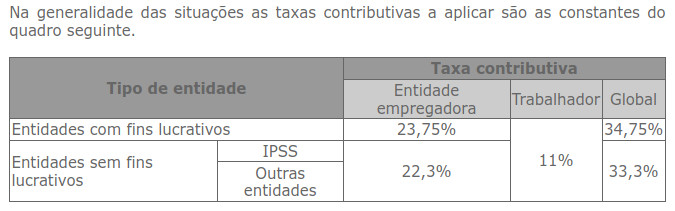
\includegraphics[width=.6\textwidth,left]{./image/SGS/Contribuicoes_1.jpg}
	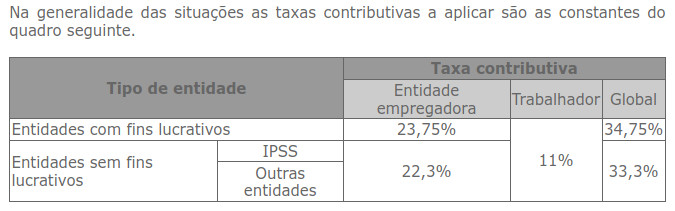
\includegraphics[scale=.5]{./image/SGS/Contribuicoes_1.jpg}
	\caption{Contribuições para SGS}
\end{figure}
\textbf{Exemplo:}
\newline
Vencimento de 1000Eur será descontado 11\% para a Segurança Social, ficando com $1000\times (1-0,11)=890Eur$ e a empresa desconta para o exemplo de 23,75\%, $1000\times 0,2375=237,5Eur$, ao todo será descontado $110+237,5=347,5Eur$, ou seja, todos os messes um trabalhador que ganhe 1000Eur desconta para a Segurança Social direto e indiretamente \textbf{347,5Eur}.
\emptyline
Na realidade o vencimento neste exemplo do cidadão devia ser de \textbf{1237,5Eur}, ou seja, é prejudicado nos seus descontos na quantia de 237,5Eur [23,75\%] pois não são considerados como pessoais. \\
A circulação deste capital passa despercebido e usado pelo estado para seus gastos, sendo o cidadão sua fonte, sem nenhum proveito, a não ser que talvez as empresas depois recebem ajudas através desta receita.
\emptyline
Em Geral a receita laboral de um cidadão é quase três oitavos $23,75\%+11\%=34,75\%$ depois dos respetivos descontos [1000Eur \textit{vs} 347,5Eur].
\emptyline
Estas contas são feitas sem considerar qualquer subsidio de alimentação.
\emptyline
\textcolor{green}{\small [ link: \quad http://www.seg-social.pt/trabalhadores-por-conta-de-outrem ]}
\subsection{Trabalhadores Independentes}
%%%%%%%%%%%%%%%%%%%%%%%%%%%%%%%%%%%%%%%%%%%%%%%%%%%%%%%%%%%%%%%%%
\qquad Este tipo de contribuinte em princípio pode definir seus descontos numa dada margem, e é aliciante para as empresas pois não tem qualquer responsabilidade, este acarreta toda a responsabilidade de descontos e despesas, no entanto em princípio ira ganhar mais do que o trabalhador por conta de outrem, mas descontando muito menos e prejudicado a longo prazo devido a concorrência, a não ser que desconte a totalidade de $23,75\%+11\%=34,75\%$ e ainda obter um vencimento superior ao seu equivalente de trabalhador por conta de outrem.
Os exemplos são trabalhadores a recibos verdes, subcontratados e a trabalho temporário.
\subsection{Precariedade}
%%%%%%%%%%%%%%%%%%%%%%%%%%%%%%%%%%%%%%%%%%%%%%%%%%%%%%%%%%%%%%%%%
\qquad Nenhum cidadão devia aceitar qualquer trabalho que ganhe menos que \; $ \mbox{\Large $ \frac{635Eur}{0,65}\approx 977Eur $ } $ para se dizer que leva uma vida sustentável, pois o salário mínimo nacional é de 635Eur, e se ficar em \textit{lay off} ou \textit{desempregado}, como demonstrado:
\emptyline
\hspace*{.3cm} $635\times(1-0,11)\approx566Eur$,\hspace*{1cm} $635\times(0,3475)\approx220Eur$,\hspace*{1cm} $\frac{635\times14}{12}\times0,65 \approx 482Eur$,
\emptyline
estará a trabalhar gratuitamente, só ira receber \textbf{566Eur} com descontos de \textbf{220Eur}, ou seja um escravo do estado. No caso de \textit{lay-off ou desemprego} recebera apenas 482Eur.\\
Em princípio qualquer remuneração será deduzido por: $Vencimento \times (1-0,11) \times (1-0,23) - Combustivel\times 0,61 = Rendimento \, Liquido$, pois tudo também leva \textit{IVA} e a taxa de combustível.
\emptyline
\textbf{Exemplo} (\textit{indivíduo com salário mínimo nacional}) \; \textbf{:}
\emptyline
1. vencimento = 635Eur e 0Eur gasolina mensal \\
\hspace*{1cm} $635Eur \times (1-0,11) \times (1-0,23) - 0Eur \times 0,61 = 435Eur$ \\
2. vencimento = 635Eur e 80Eur gasolina mensal \\
\hspace*{1cm} $635Eur \times (1-0,11) \times (1-0,23) - 80Eur \times 0,61 = 386Eur$ \\
3. vencimento = 635Eur e 150Eur gasolina mensal \\
\hspace*{1cm} $635Eur \times (1-0,11) \times (1-0,23) - 150Eur \times 0,61 = 343Eur$,
\emptyline
mas ainda não acaba aqui a pintura negra, supondo agora que o cidadão não tem caro, ou seja, recebe limpos 435Eur, ainda vai ter que pagar taxa água e saneamento (mínimo 11,3Eur) e taxa de luz (mínimo 8Eur). Fica com 415,7Eur, para piorar vamos supor que tem habitação e têm que pagar IMI (mínimo 11Eur/mês).
Se este exemplo tiver um empréstimo de habitação e ou um veiculo chegamos a conclusão que não pode se alimentar, o que será muito bom para a dieta, e doenças.
\emptyline
Concluindo que no estado presente de trabalho só é benéfico se pertencermos aos membros de órgãos estatuários ou político, pois não tem encargos do estado e aufere de regalias e vencimentos mínimo de cinco vezes e até dez vezes superior ao salário mínimo nacional, também existindo casos excecionais de vinte e para cima a mais o salário mínimo nacional. Sendo que esta profissão existe apenas por tráfico de influências e não igualdade ou equidade, muito menos competência, como demonstrado com esta pandemia na qual suas soluções para os problemas são solidariedade.
\subsection{Mudança}
%%%%%%%%%%%%%%%%%%%%%%%%%%%%%%%%%%%%%%%%%%%%%%%%%%%%%%%%%%%%%%%%%
\qquad Já é conhecido que em \textsf{2025}, 75\% da classe trabalhadora vai pertencer a geração \textbf{Y}, e o quadro do futuro de trabalho esta cada vez mais centrado a volta do desenvolvimento tecnológico, as sociedades vão ter que acompanhar o ritmo de crescimento, e a União Europeia e seus membros reconhecem esta tendência e a necessidade de formação e treino destas competências nos trabalhadores Europeus, sendo o projeto \textit{industria 4.0} uma destas ferramentas.
\begin{figure}[H]
	\centering
	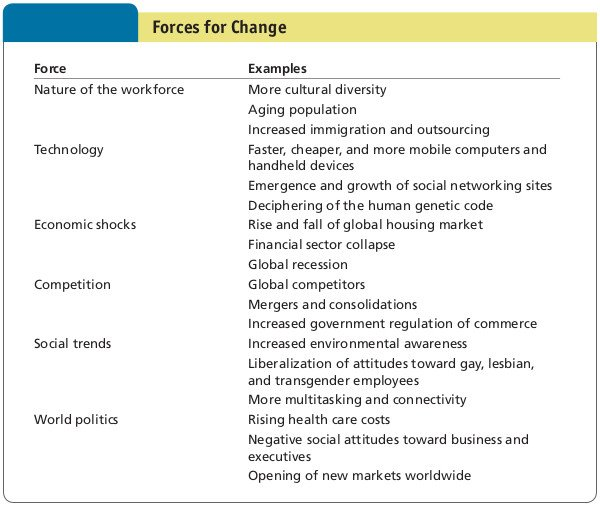
\includegraphics[scale=0.52]{./image/Change/Forces_for_Change.jpg}
	\caption{Forças para a Mudança \cite{book-7}}
\end{figure}
Empresas de todo tipo e dimensão estão a ser enfrentados com a questão de como podem assegurar o fornecimento de líderes com as competências, habilidades e visão estratégica adequadas para obter o sucesso. Ignorando a velha mentalidade de que certos indivíduos nascem para liderar, muitas empresas acreditam que a liderança pode ser desenvolvida numa forma pro-ativa e de forma sistemática. \cite{book-6}
\emptyline
A liderança assume um papel importante na mudança de cultura dentro das organizações e requer estar sempre em constante adaptação ao seu meio ambiente. Como sugere a liderança \textit{VUCA}, que representa Volatilidade, incerteza (uncertainty), complexidade e ambiguidade. Volatile porque não é estático esta e em constante mudança, incerteza na previsão do futuro, complexo com sistemas cada vez mais sofisticados que requer competências adequadas e ambíguo com problemas difícil de identificar, pouca informação de alternativas, sem se saber as consequências.
\begin{figure}[H]
	\centering
	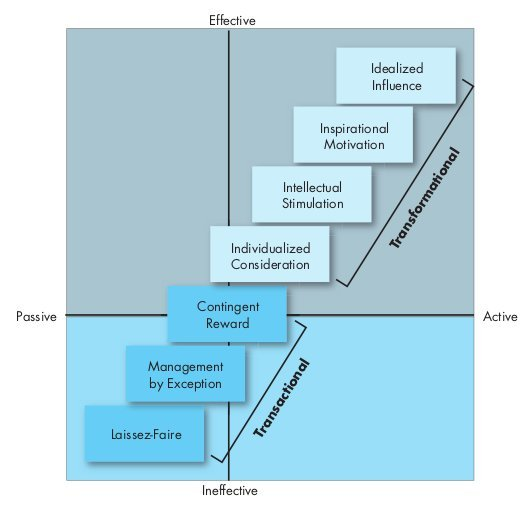
\includegraphics[scale=0.52]{./image/Leadership/Leadership_Models.jpg}
	\caption{Modelos da Liderança \cite{book-2}}
\end{figure}
Este trabalho esta focado no futuro do trabalho, gestão de carreira e marketing pessoal, no entanto abordar as matérias da gestão de mudança, a planeada (Modelo Kurt Lewin) e a emergente, os tipos de lideres, seus estilos e abordagens, também os modelos criados (Modelo Blake \& Mouton, Hersey \& Blanchard) são ferramentas úteis para nos orientar nos nossos comportamentos em diferentes contextos e determinar as atitudes a tomar com o nosso grupo ou equipa de forma a poder alcançar os objetivos e uma visão, ou seja garantir a sobrevivência e prosperidade da organização.
\begin{figure}[H]
	\centering
	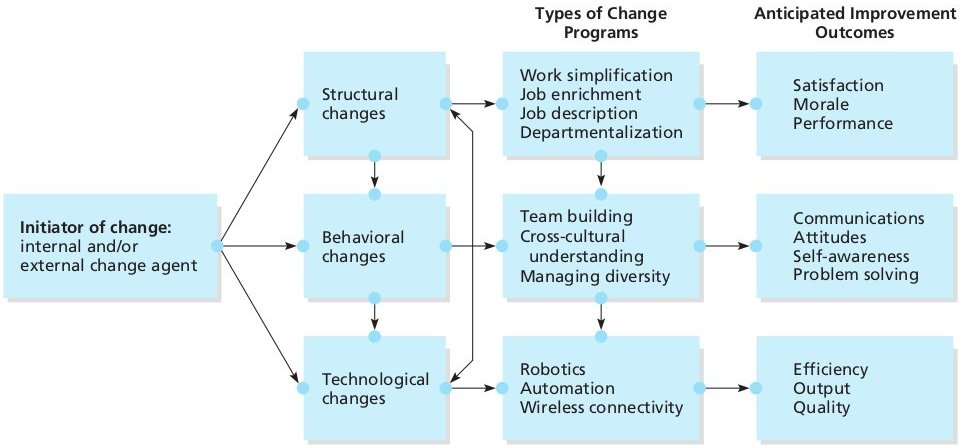
\includegraphics[scale=0.52]{./image/Change/Three_Change_Approaches.jpg}
	\caption{Três formas de mudar \cite{book-6}}
\end{figure}
 % Introduction
\section{Law}
%%%%%%%%%%%%%%%%%%%%%%%%%%%%%%%%
\subsection{Exponents}
\begin{enumerate}
	\item
	\[a^m \; \times \; a^n \; = a^{m+n} \qquad (m, \; n \in \mathbb{N})\] \[a^m \; \times \; a^n \; = a^{m+n} \qquad (m, \; n \in \mathbb{Z}; \; a \neq 0, \; if \quad m \quad or \quad n \; < \; 0)\]
	\item
	\[\frac{a^m}{a^n}=a^{m-n} \qquad (m, \; n \in \mathbb{Z}; \; a \in \mathbb{R}; \; a \neq 0)\]
	\item
	\[(ab)^m \; = \; a^m \; b^m \qquad (m \in \mathbb{Z})\]
	\item
	\[(a^m)^n \; = \; a^{mn} \qquad (m, \; n \in \mathbb{Z})\]
\end{enumerate}
%%%%%%%%%%%%%%%%%%%%%%%%%%%%%%%%
\subsection{Rational Exponents}
\begin{enumerate}
	\item
	\[a^r \; \times \; a^t \; = \; a^{r+t} \qquad (a \; > \; 0; \quad r, \; t \in \mathbb{Q})\]
	\item
	\[\frac{a^r}{a^t}=a^{r-t} \qquad (a \; > \; 0; \quad r, \;t \in \mathbb{Q})\]
	\item
	\[(a^t)^r \; = \; a^{tr} \qquad (a \; > \; 0, \quad t, \; r \in \mathbb{Q})\]
	\item
	\[(ab)^t \; = \; a^t \; b^t \; ; \quad \left(\frac{a}{b}\right)^t \; = \; \frac{a^t}{b^t} \; ; \qquad (a, \; b \; > \; 0, \quad t \in \mathbb{Q})\]
	\[\hspace{1cm} and :\]
	\[\hspace{3cm} a^t \; b^t \; = \; (ab)^t \qquad and \qquad \frac{a^t}{b^t} \; = \; \left(\frac{a}{b}\right)^t\]
\end{enumerate}
%%%%%%%%%%%%%%%%%%%%%%%%%%%%%%%%
\subsection{Distributive law}
\[a(b \; + \; c) \; = \; ab \; + \; ac\]
\begin{align*}
	(a \; + \; b)(c \; + \; d) \; &= \; (a \; + \; b)c \; + \; (a \; + \; b)d \\
	&=ac \; + \;bc \; + \; ad \; + \; bd
\end{align*}
\[A^2 \; - \; B^2 \; = \; (A \; - \; B)(A \; + \; B)\]
%%%%%%%%%%%%%%%%%%%%%%%%%%%%%%%%
\subsection{Commutative law}
\[ab \; = \; ba\]
%%%%%%%%%%%%%%%%%%%%%%%%%%%%%%%%
%%%%%%%%%%%%%%%%%%%%%%%%%%%%%%%%%%%%%%%%%%%%%%%%%%%%%%%%%%%%%%%%%%%%%
 % Revisão da Literatura
\section{Conclusão}
%%%%%%%%%%%%%%%%%%%%%%%%%%%%%%%%%%%%%%%%%%%%%%%%%%%%%%%%%%%%%%%%%
\qquad O futuro do trabalho passa por adquirir novas competências, e conseguir adaptação as novas tendências, a procura de oportunidades e valorização pessoal uma mais valia. Já foi demonstrado que é importante desenvolvermos tanto as nossas metodologias de trabalho como a experiência para estarmos preparados para enfrentar os desafios que possam surgir. \\
\\
Ninguém sabe o futuro, muito menos o imprevistos, cabe as novas gerações decidir, a liberdade acho que é algo que todos desejam, a estabilidade e segurança, mas não só depende de nós, o planeta terra, a galáxia e o universo tem palavra soberana.\\
\\
Considero a humildade e gratidão um atributo fundamental, saber que estamos sujeitos a forças maiores e respeitar essas fronteiras, historicamente isso foi comprovado vezes sem conta, e hoje é outra prova disso, como a pandemia.\\
\\
Gerações após gerações existe uma concentração tremenda muito focada com uma visão míope, um convite para o desastre. Sabe-se lá se temos cura. No entanto temos que ter esperança que haja visão e iluminação.
Esta conversa até parece religiosa, mas nada disso.\\
\\
Ainda muitas conclusões pode-se tirar acerca do futuro do trabalho e marketing pessoal, que não entra nos parâmetros deste relatório e discussão, o desenvolvimento é uma forma de enriquecimento mais rápido e eficaz, com contornos sociais complicados, da a entender que vai haver um excesso de produção sem clientes á vista, um problema de reciclagem e sobrevivência, talvez devia haver uma preocupação na  regulamentação.\\
\\
O ensino talvez esta a ficar desadequado para nossos tempos, não incluindo as ferramentas necessárias na formação e treino, o tempo de retenção dos estudantes excessivo, que provoca colisões entre gerações, especialmente num país pequeno com uma cultura estática, sendo quase impossível obter os resultados esperados caindo na decadência social e económica no seu geral, etc, etc, etc.\\
\\
No meu ver \textcolor{green}{Portugal} deixou de ser um país mas uma fábrica, as competências uma forma de sobreviver no sentido de estar numa escala mais favorável, dai que a solução de mudar para uma sociedade onde o valor individual depende das competências origina a juventude fugir deste sistema instalado.\\
\\
Abaixo link de apanhado de dados utilizados para este relatório:\\ \textcolor{green}{\small [ https://padlet.com/sergio1020881/xih48fe75koesxdg ]}
\begin{comment}
Não conheço nenhuma geração que não tenha passado por dificuldades tremendas, episódios horrendos. Parece existe mudança mas fica tudo igual, o sistema já esta implementado. \\
Para sobreviver temos de nos adaptar e competir, mas a maquina é a mesma. A gerência parece estática e firme é uma herança perpetua de desigualdade. \\
\end{comment}
%%%%%%%%%%%%%%%%%%%%%%%%%%%%%%%%%%%%%%%%%%%%%%%%%%%%%%%%%%%%%%%%%
 % Organização
\begin{figure}[H]
	\centering
	\begin{multicols}{2}
	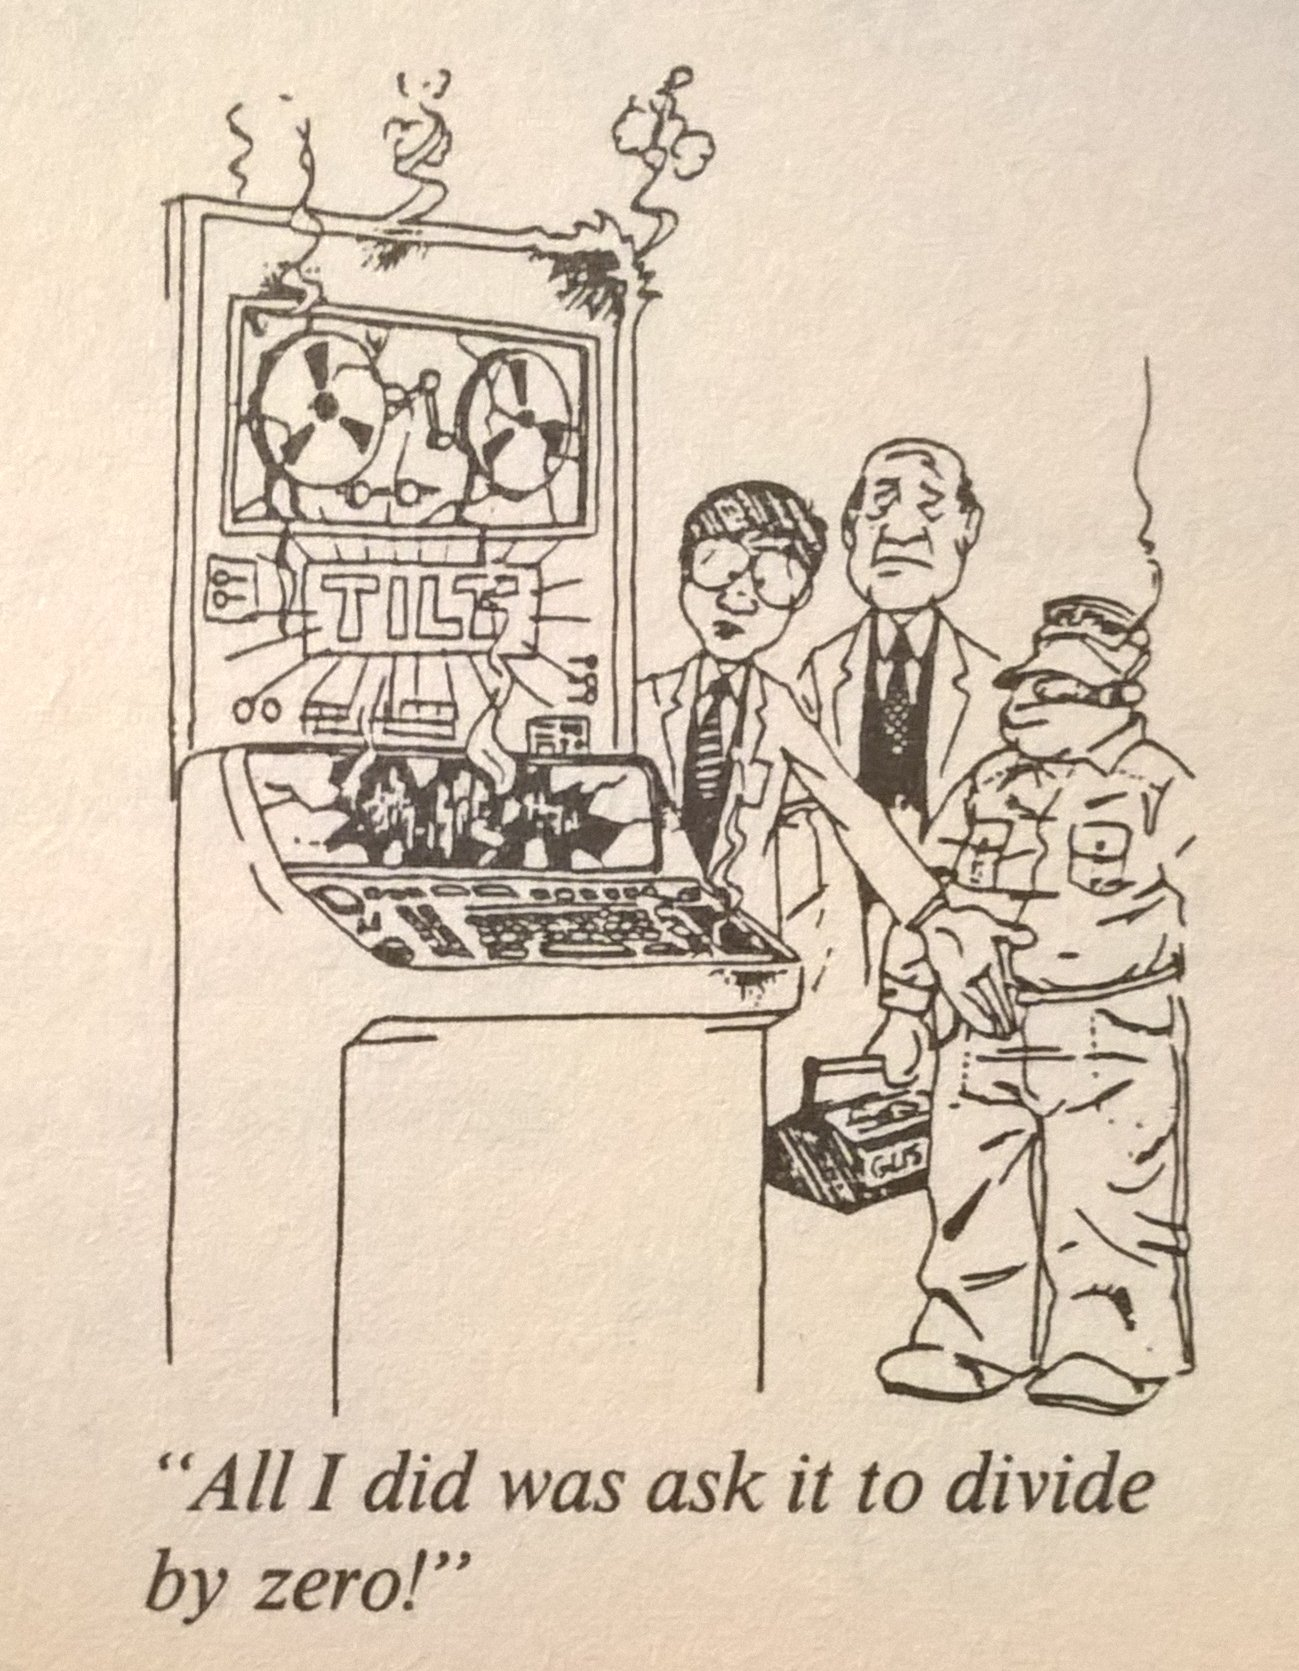
\includegraphics[scale=0.2, left]{dividebyzero.jpg}
	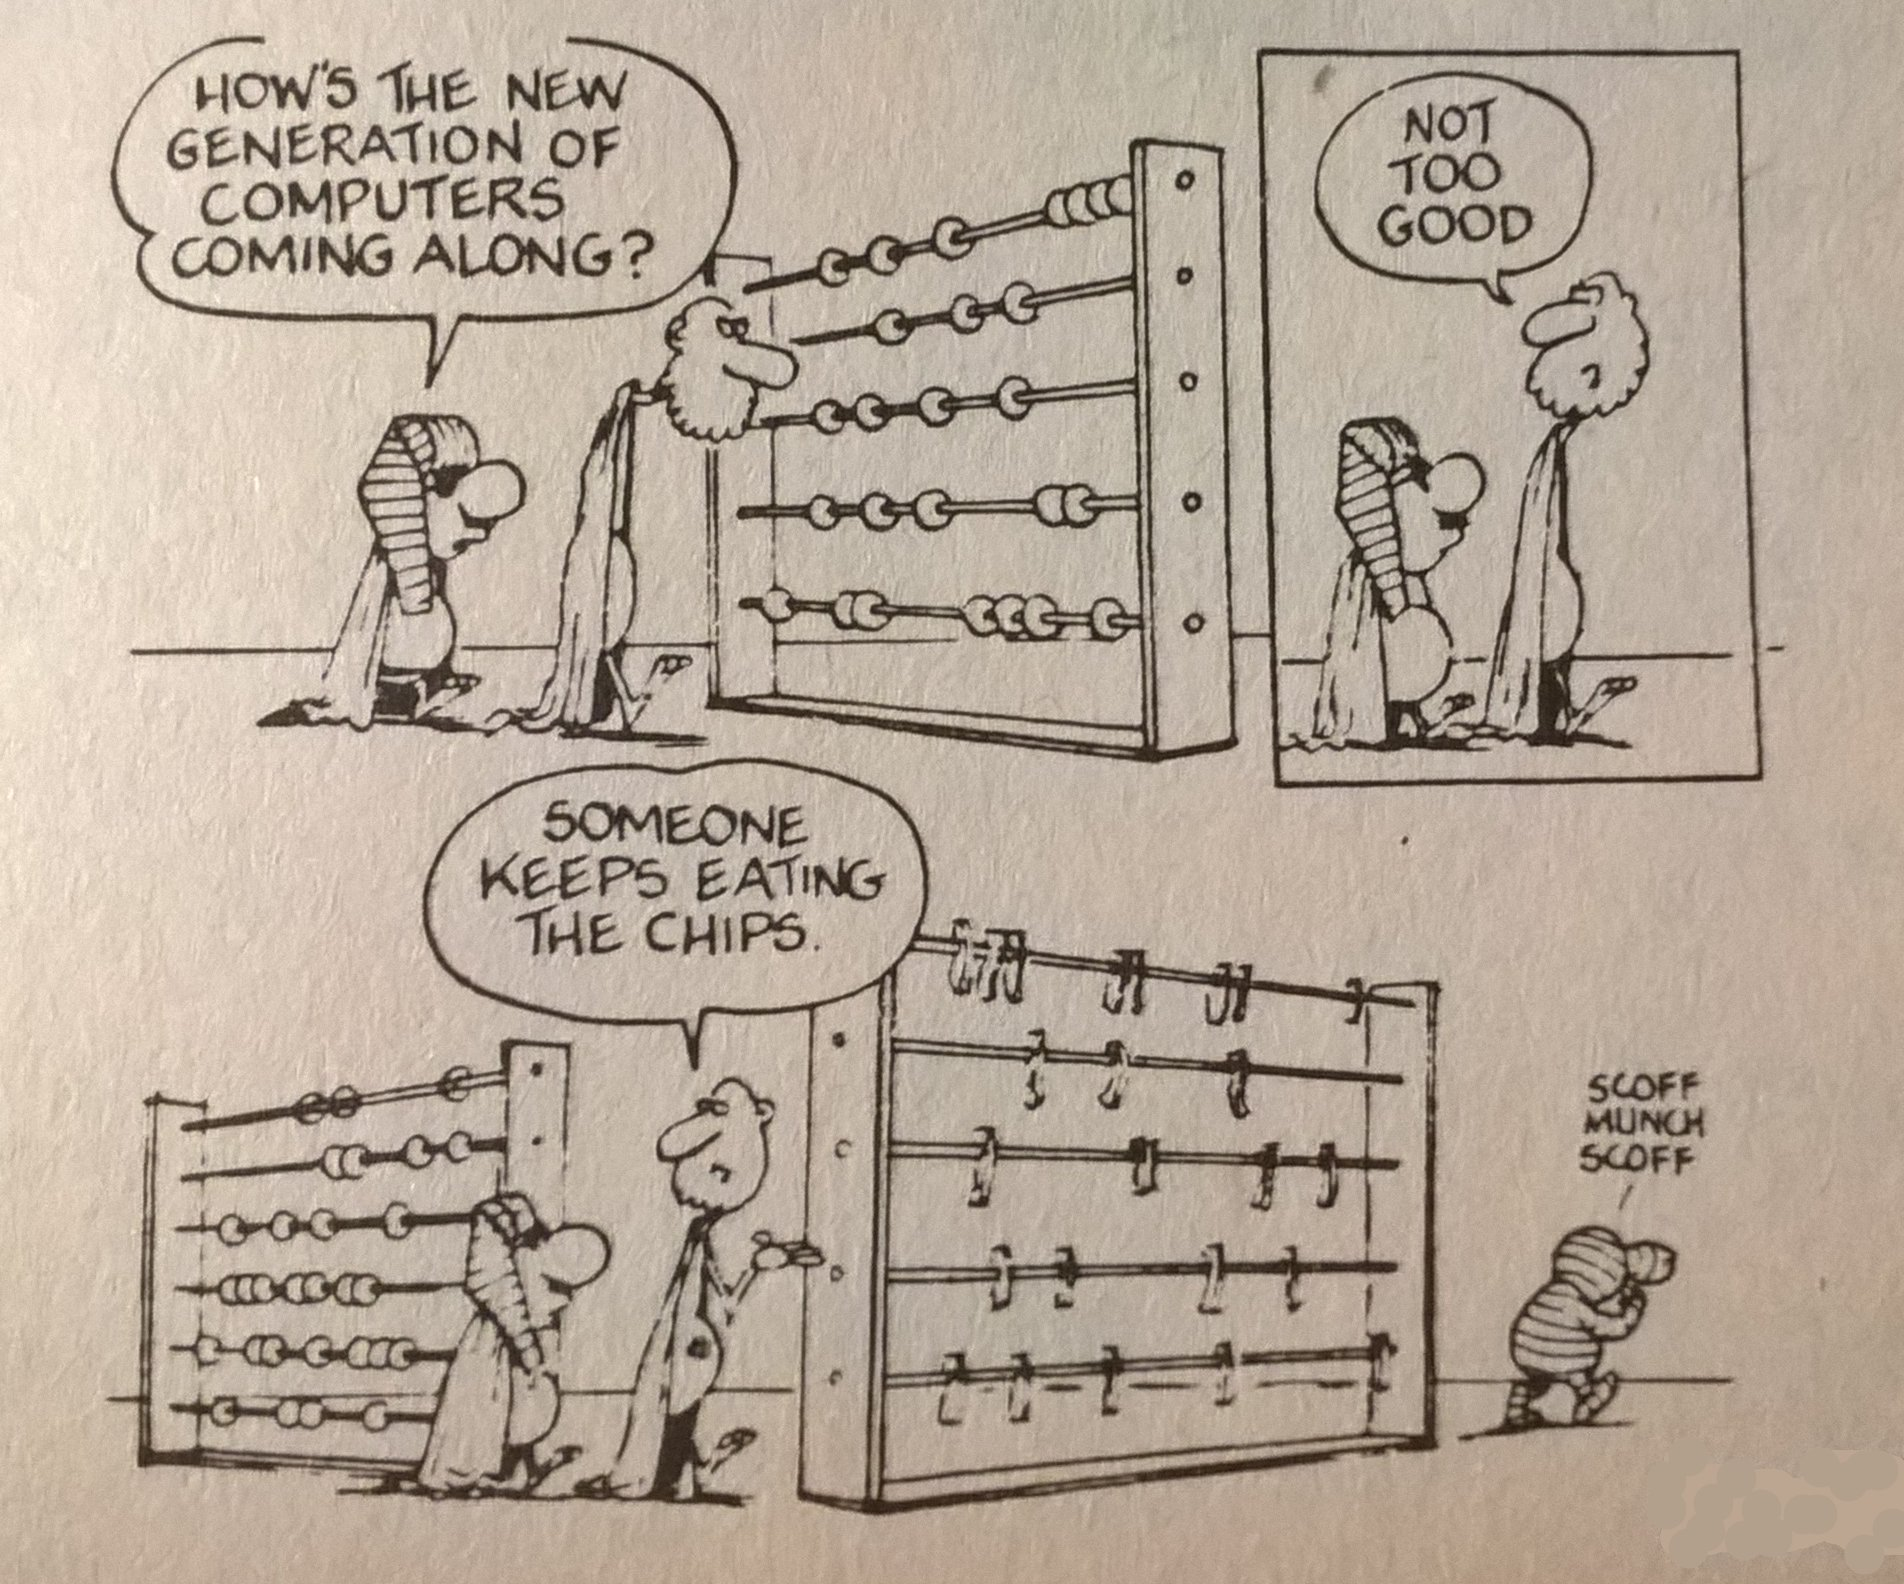
\includegraphics[scale=0.12, right]{newgencomputer.jpg}
	\end{multicols}
\end{figure}
\newpage
%%%%%%%%%%%%%%%%%%%%%%%%%%%%%%%%
\begin{comment}
\begin{figure}[H]
	\begin{subfigure}[h]{0.5\textwidth}
		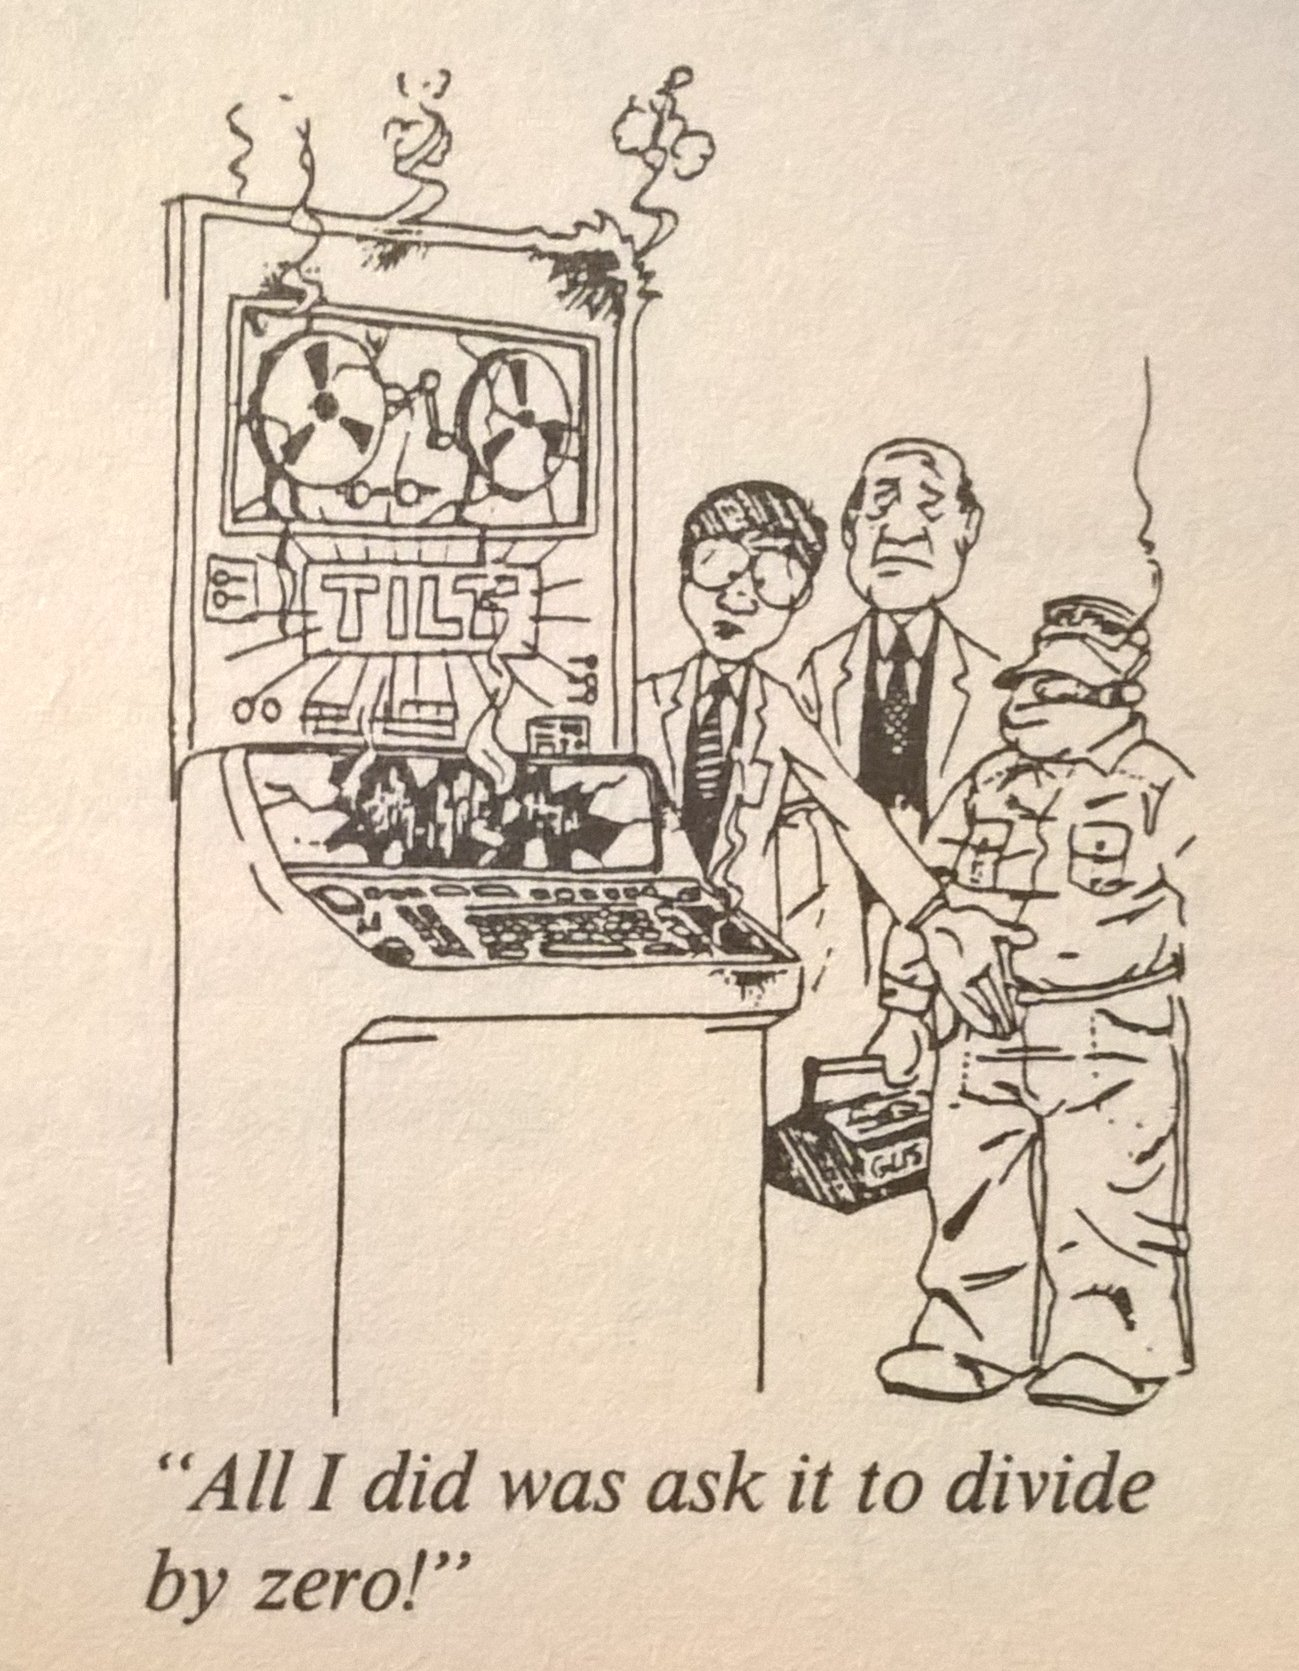
\includegraphics[scale=0.2, left]{dividebyzero.jpg}
	\end{subfigure}
	\hspace{.5cm}
	\begin{subfigure}[h]{0.5\textwidth}
		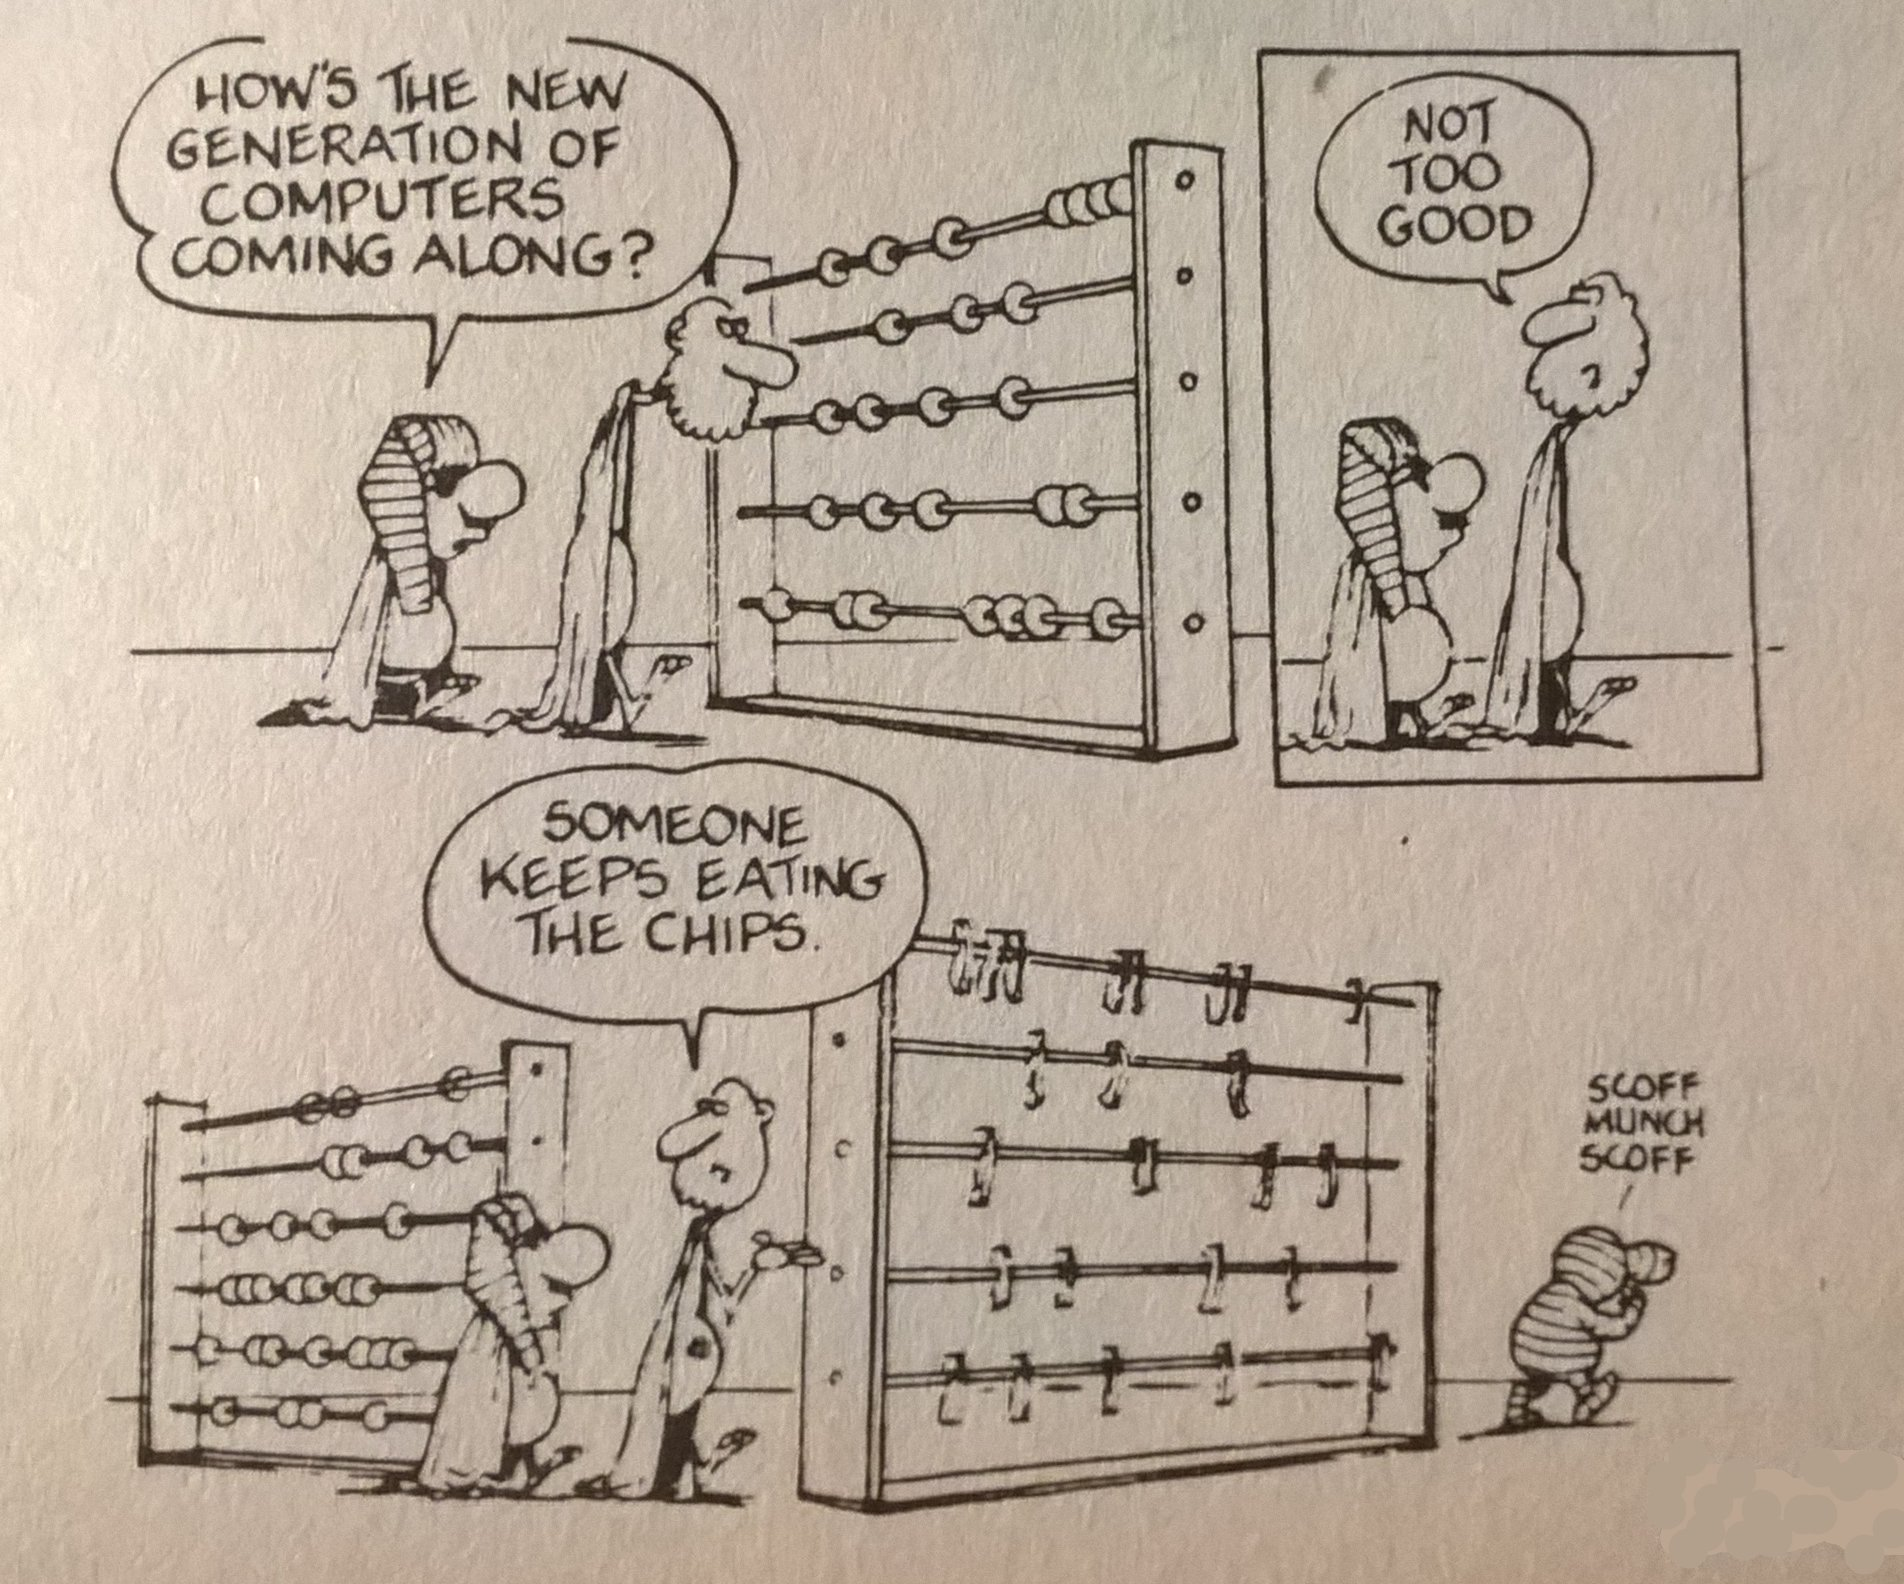
\includegraphics[scale=0.12, right]{newgencomputer.jpg}
	\end{subfigure}
\end{figure}
\end{comment}
%%%%%%%%%%%%%%%%%%%%%%%%%%%%%%%%%%%%%%%%%%%%%%%%%%%%%%%%%%%%%%%%%%%%%%%%%%%%%%%%%
 % Cultura Organizacional
\section{Examples}
\begin{minipage}{\linewidth}
	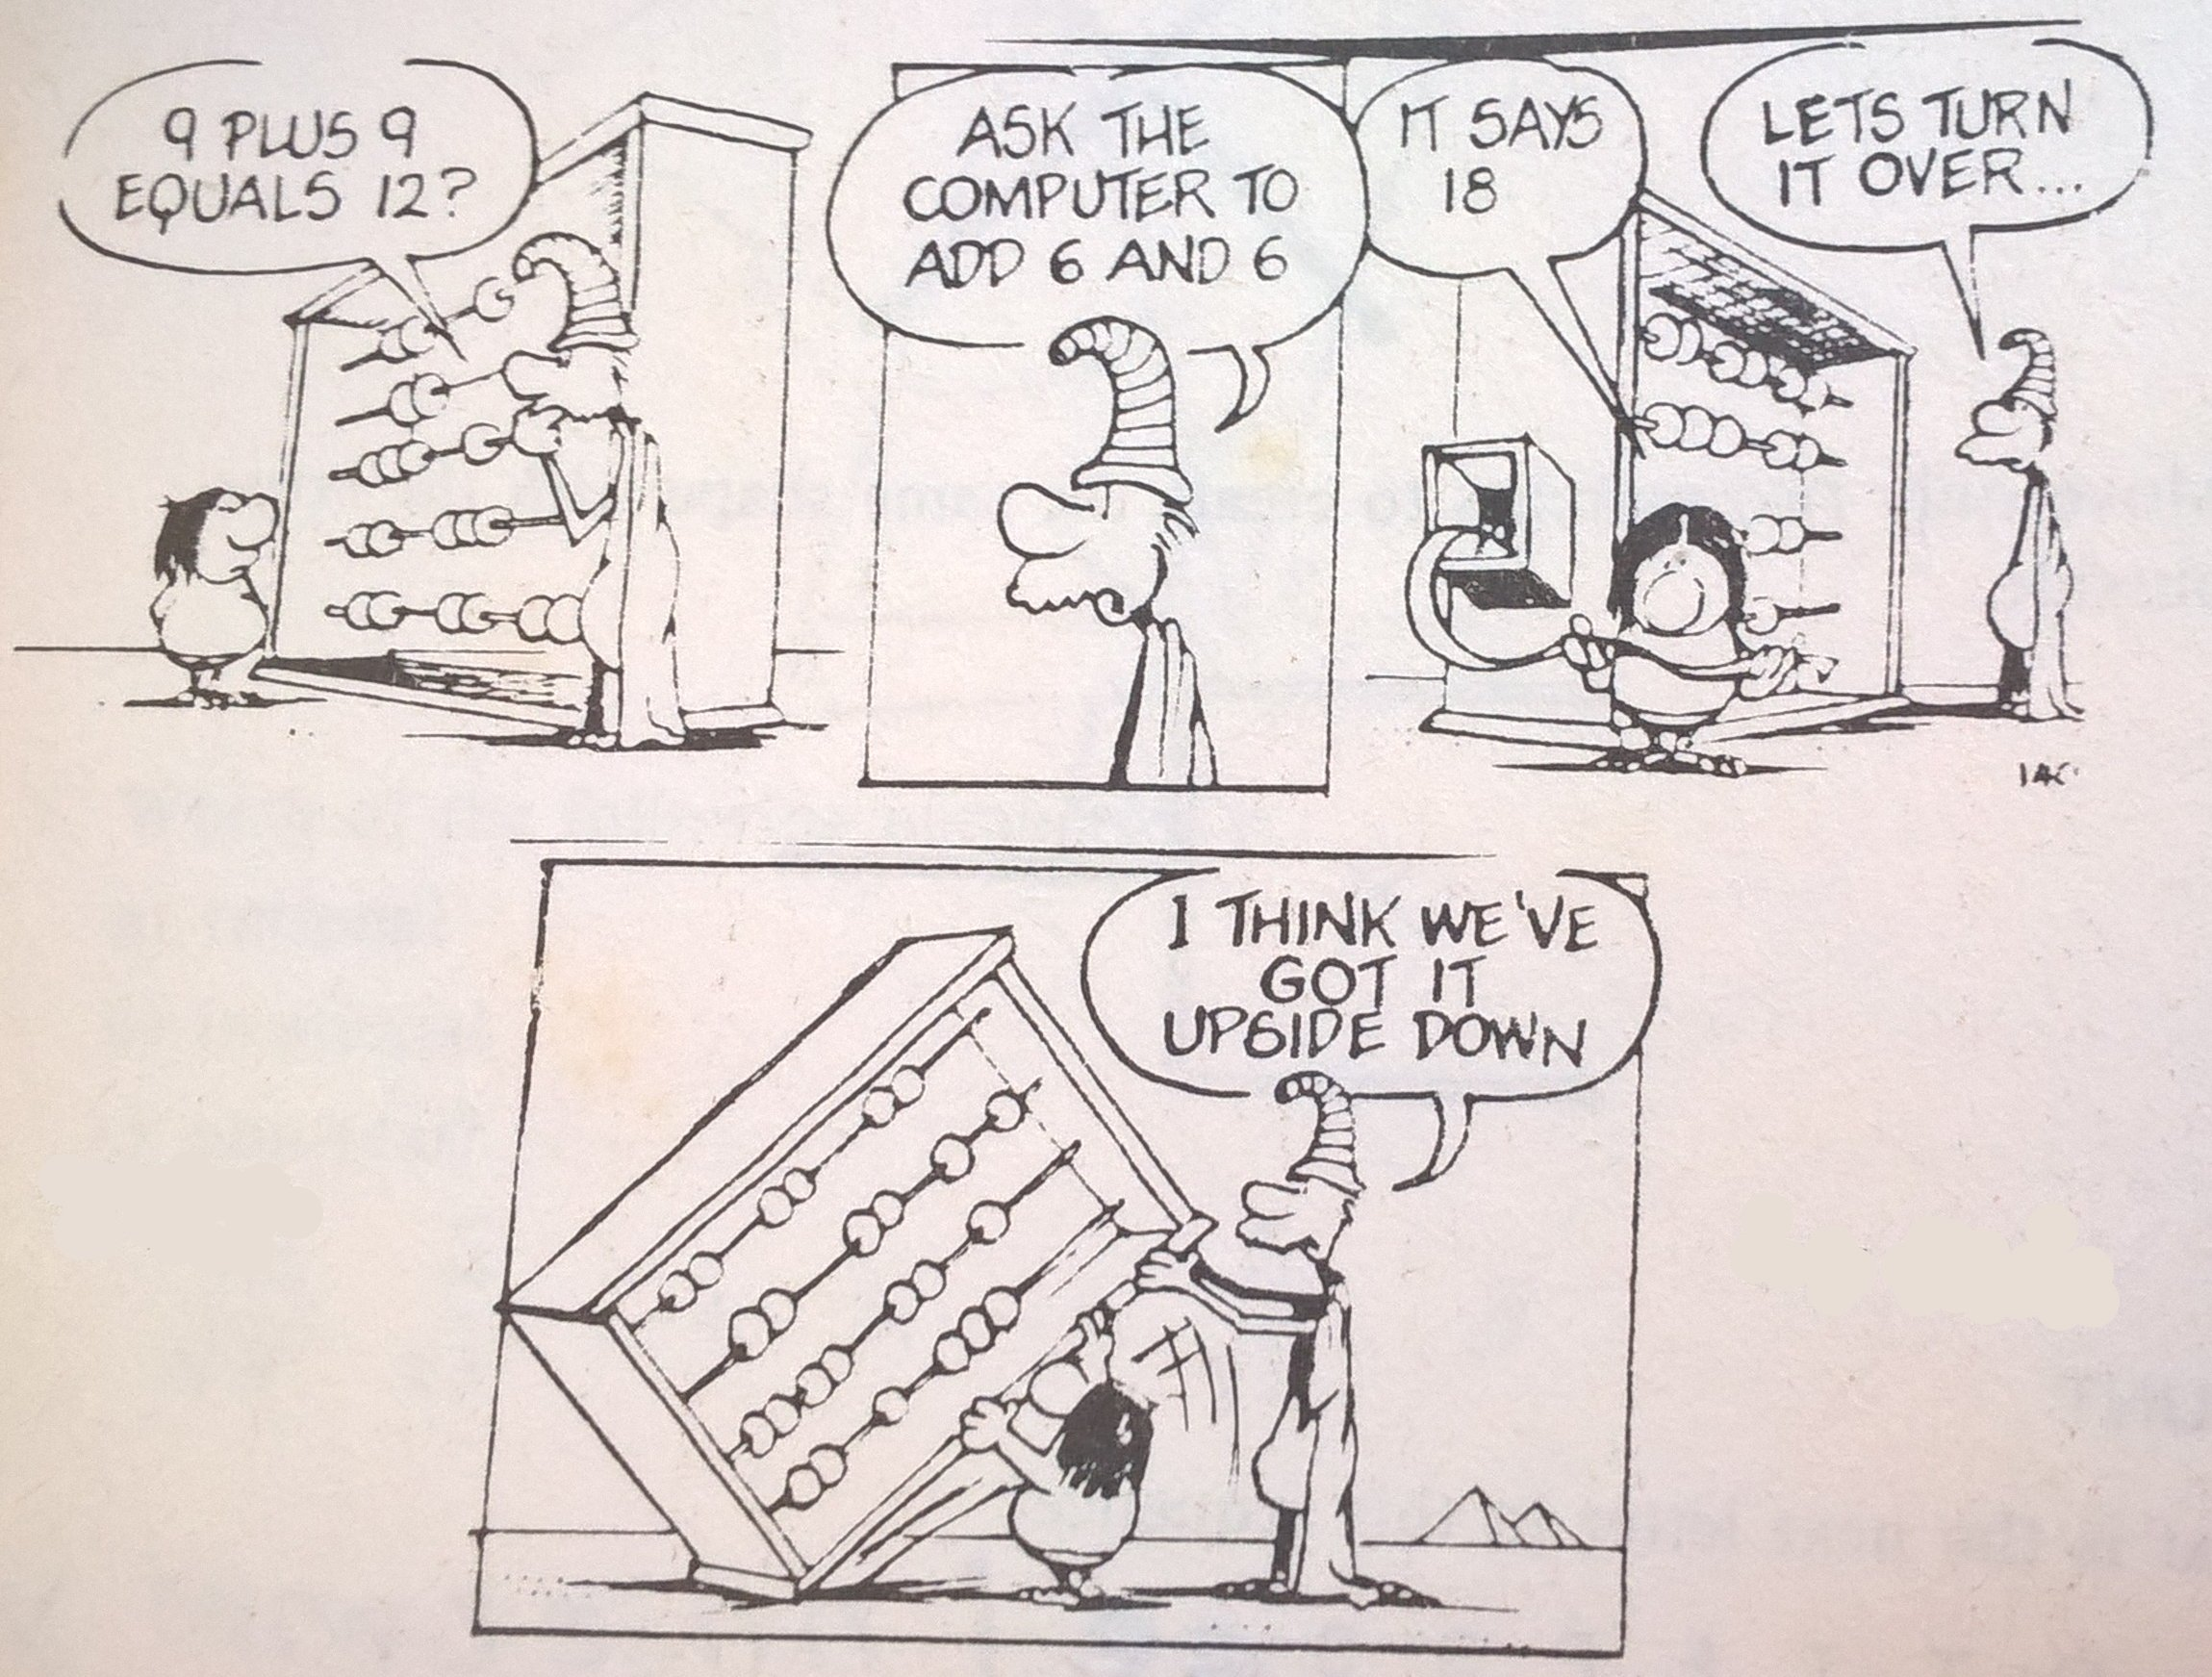
\includegraphics[scale=0.2]{./image/upsidedown.jpg}
\end{minipage}
\minipagespace{.2cm}
%%%%%%%%%%%%%%%%%%%%%%%%%%%%%%%%%%%%%%%%%%%%%%%%%%%%%%%%%%

\[\sqrt{a^2} \; = \; a \qquad (a \; > \; 0) \qquad \qquad \sqrt{a^n} \; = \; a^{\frac{n}{2}}\] \\
\[\sqrt{\frac{1}{a}} \; = \; \frac{1}{\sqrt{a}}\] \\
\[a^{\frac{m}{1}} \; = \; a^m \qquad \qquad \frac{a^m}{a^n} \; = \; a^{m-n}\] \\
\[\frac{a \; \angle \alpha^\circ \; b \; \angle \beta^\circ}{c \; \angle \gamma^\circ} \; = \; \frac{a \times b}{c} \quad \angle \; (\alpha^\circ + \beta^\circ - \gamma^\circ)\]
\\
\[If \quad a \; . \; b \; = \; 0, \quad then \quad a \; = \; 0 \quad or \quad b \; = \; 0\]
\emptyline
\begin{minipage}{0.60\linewidth}
	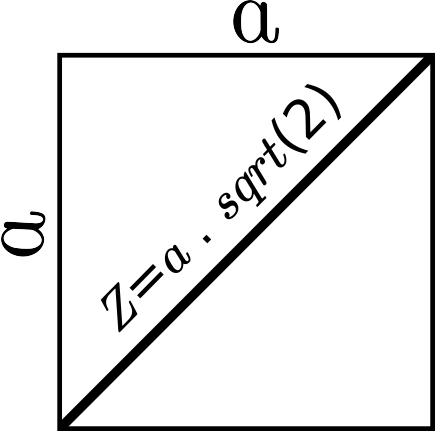
\includegraphics[scale=0.5]{./image/squareproperty.png}
\end{minipage}
\begin{minipage}[H]{0.3\linewidth}
	\textbf{Square Property} \\
	\[Z=\sqrt{a^2 \; + \; a^2}\]
	\[Z=\sqrt{2 \; a^2}\]
	\[Z=\sqrt{2} \quad \sqrt{a^2}\]
	\[Z=\sqrt{2} \quad a\]
\end{minipage}
\minipagespace{1cm}
\[a \; \angle \alpha \; + \; b \; \angle \beta \; = \; \sqrt{(a \;  \sin \alpha \; + \; b \; \sin \beta)^2 \; + \; (a \; \cos \alpha \; + \; b \; \cos \beta)^2}\] \\
and \\
\[\angle \arctan(\frac{(a \; \sin \alpha \; + \; b \; \sin \beta)}{(a \; \cos \alpha \; + \; b \; \cos \beta)})\] \\
\begin{align*}
	\lim_{s \to 0}{GH(s)} & = \lim_{s \to 0} \quad 7 \; \frac{4+3s}{5+2s+6s^2} \\ \\
	& = \lim_{s \to 0} \quad 7 \; \frac{4(1+\frac{3}{4}s)}{5(1+\frac{2}{5}s+\frac{6}{5}s^2)} \\ \\
	& = 7 \; \frac{4}{5}
\end{align*}
\begin{align*}
	y'(x) &= \ce^{4x+5} \\
	&= 4 \; \ce^{4x+5}
\end{align*}
\emptyline
%%%%%%%%%%%%%%%%%%%%%%%%%%%%%%%%
\begin{minipage}{0.80\linewidth}
	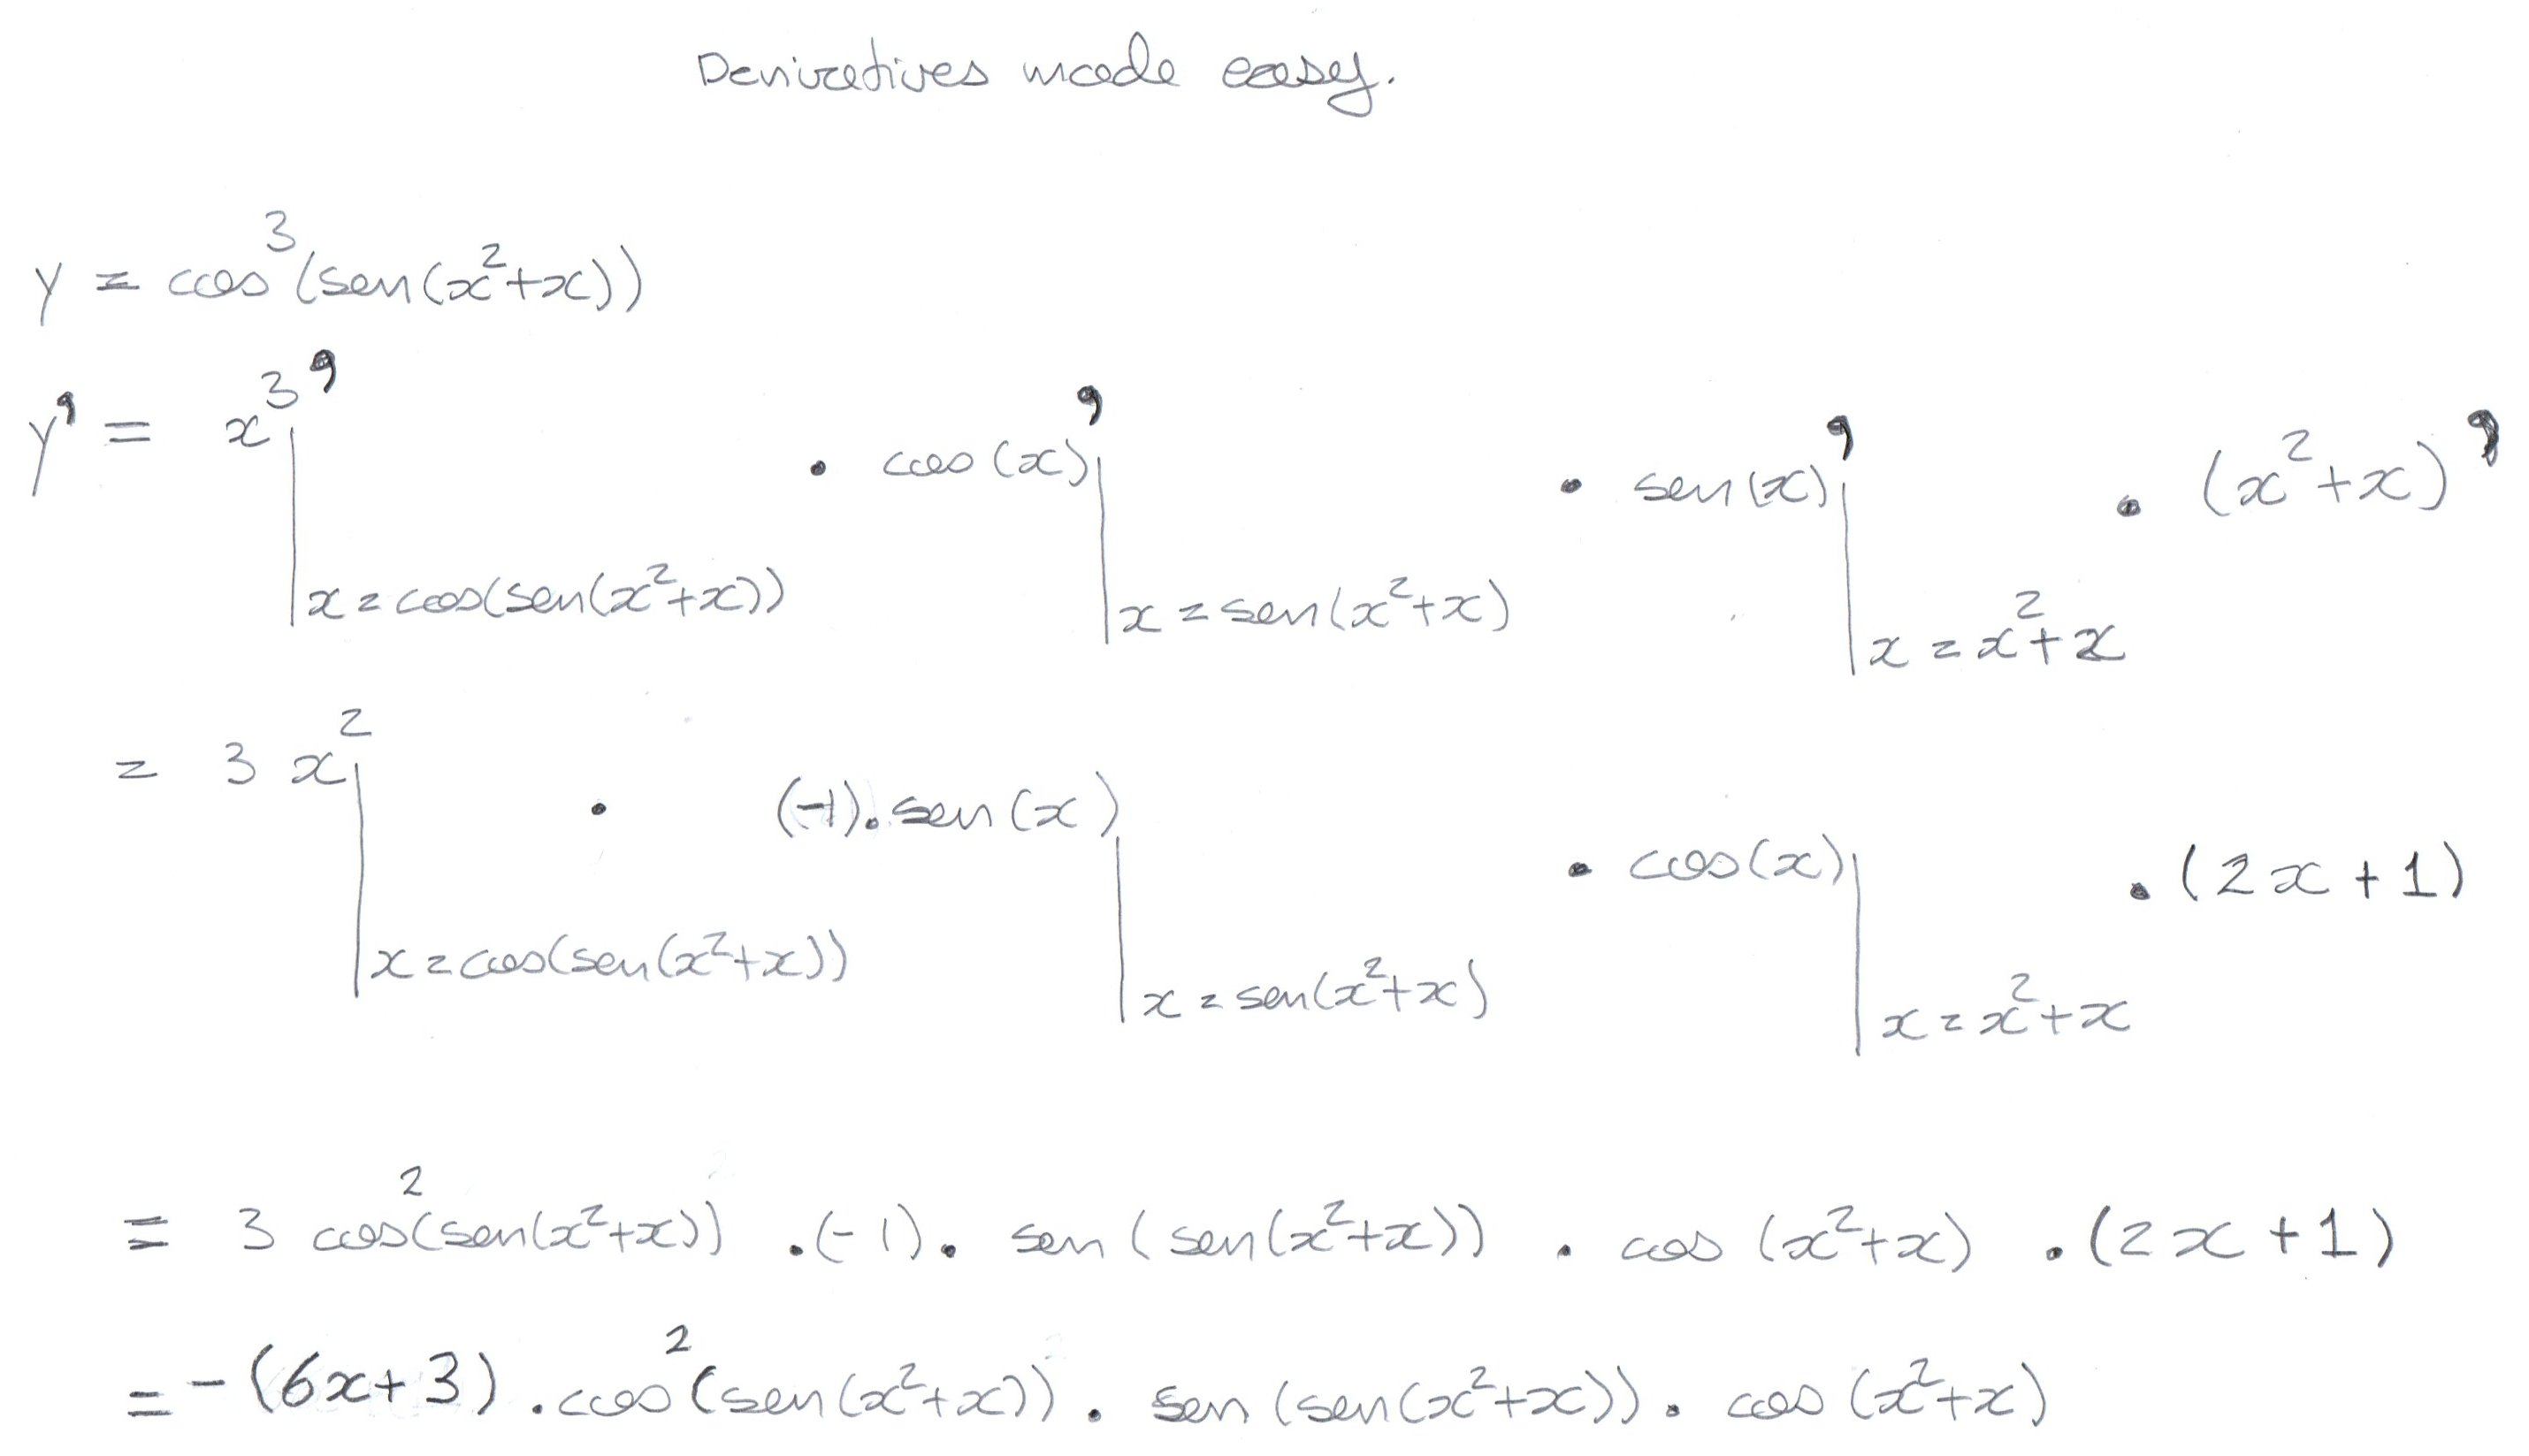
\includegraphics[scale=0.18]{./image/derivativeasy_1.jpg}
\end{minipage}
%%%%%%%%%%%%%%%%%%%%%%%%%%%%%%%%%%%%%%%%%%%%%%%%%%%%%%%%%%
\newpage
%%%%%%%%%%%%%%%%%%%%%%%%%%%%%%%%
\begin{minipage}{0.80\linewidth}
	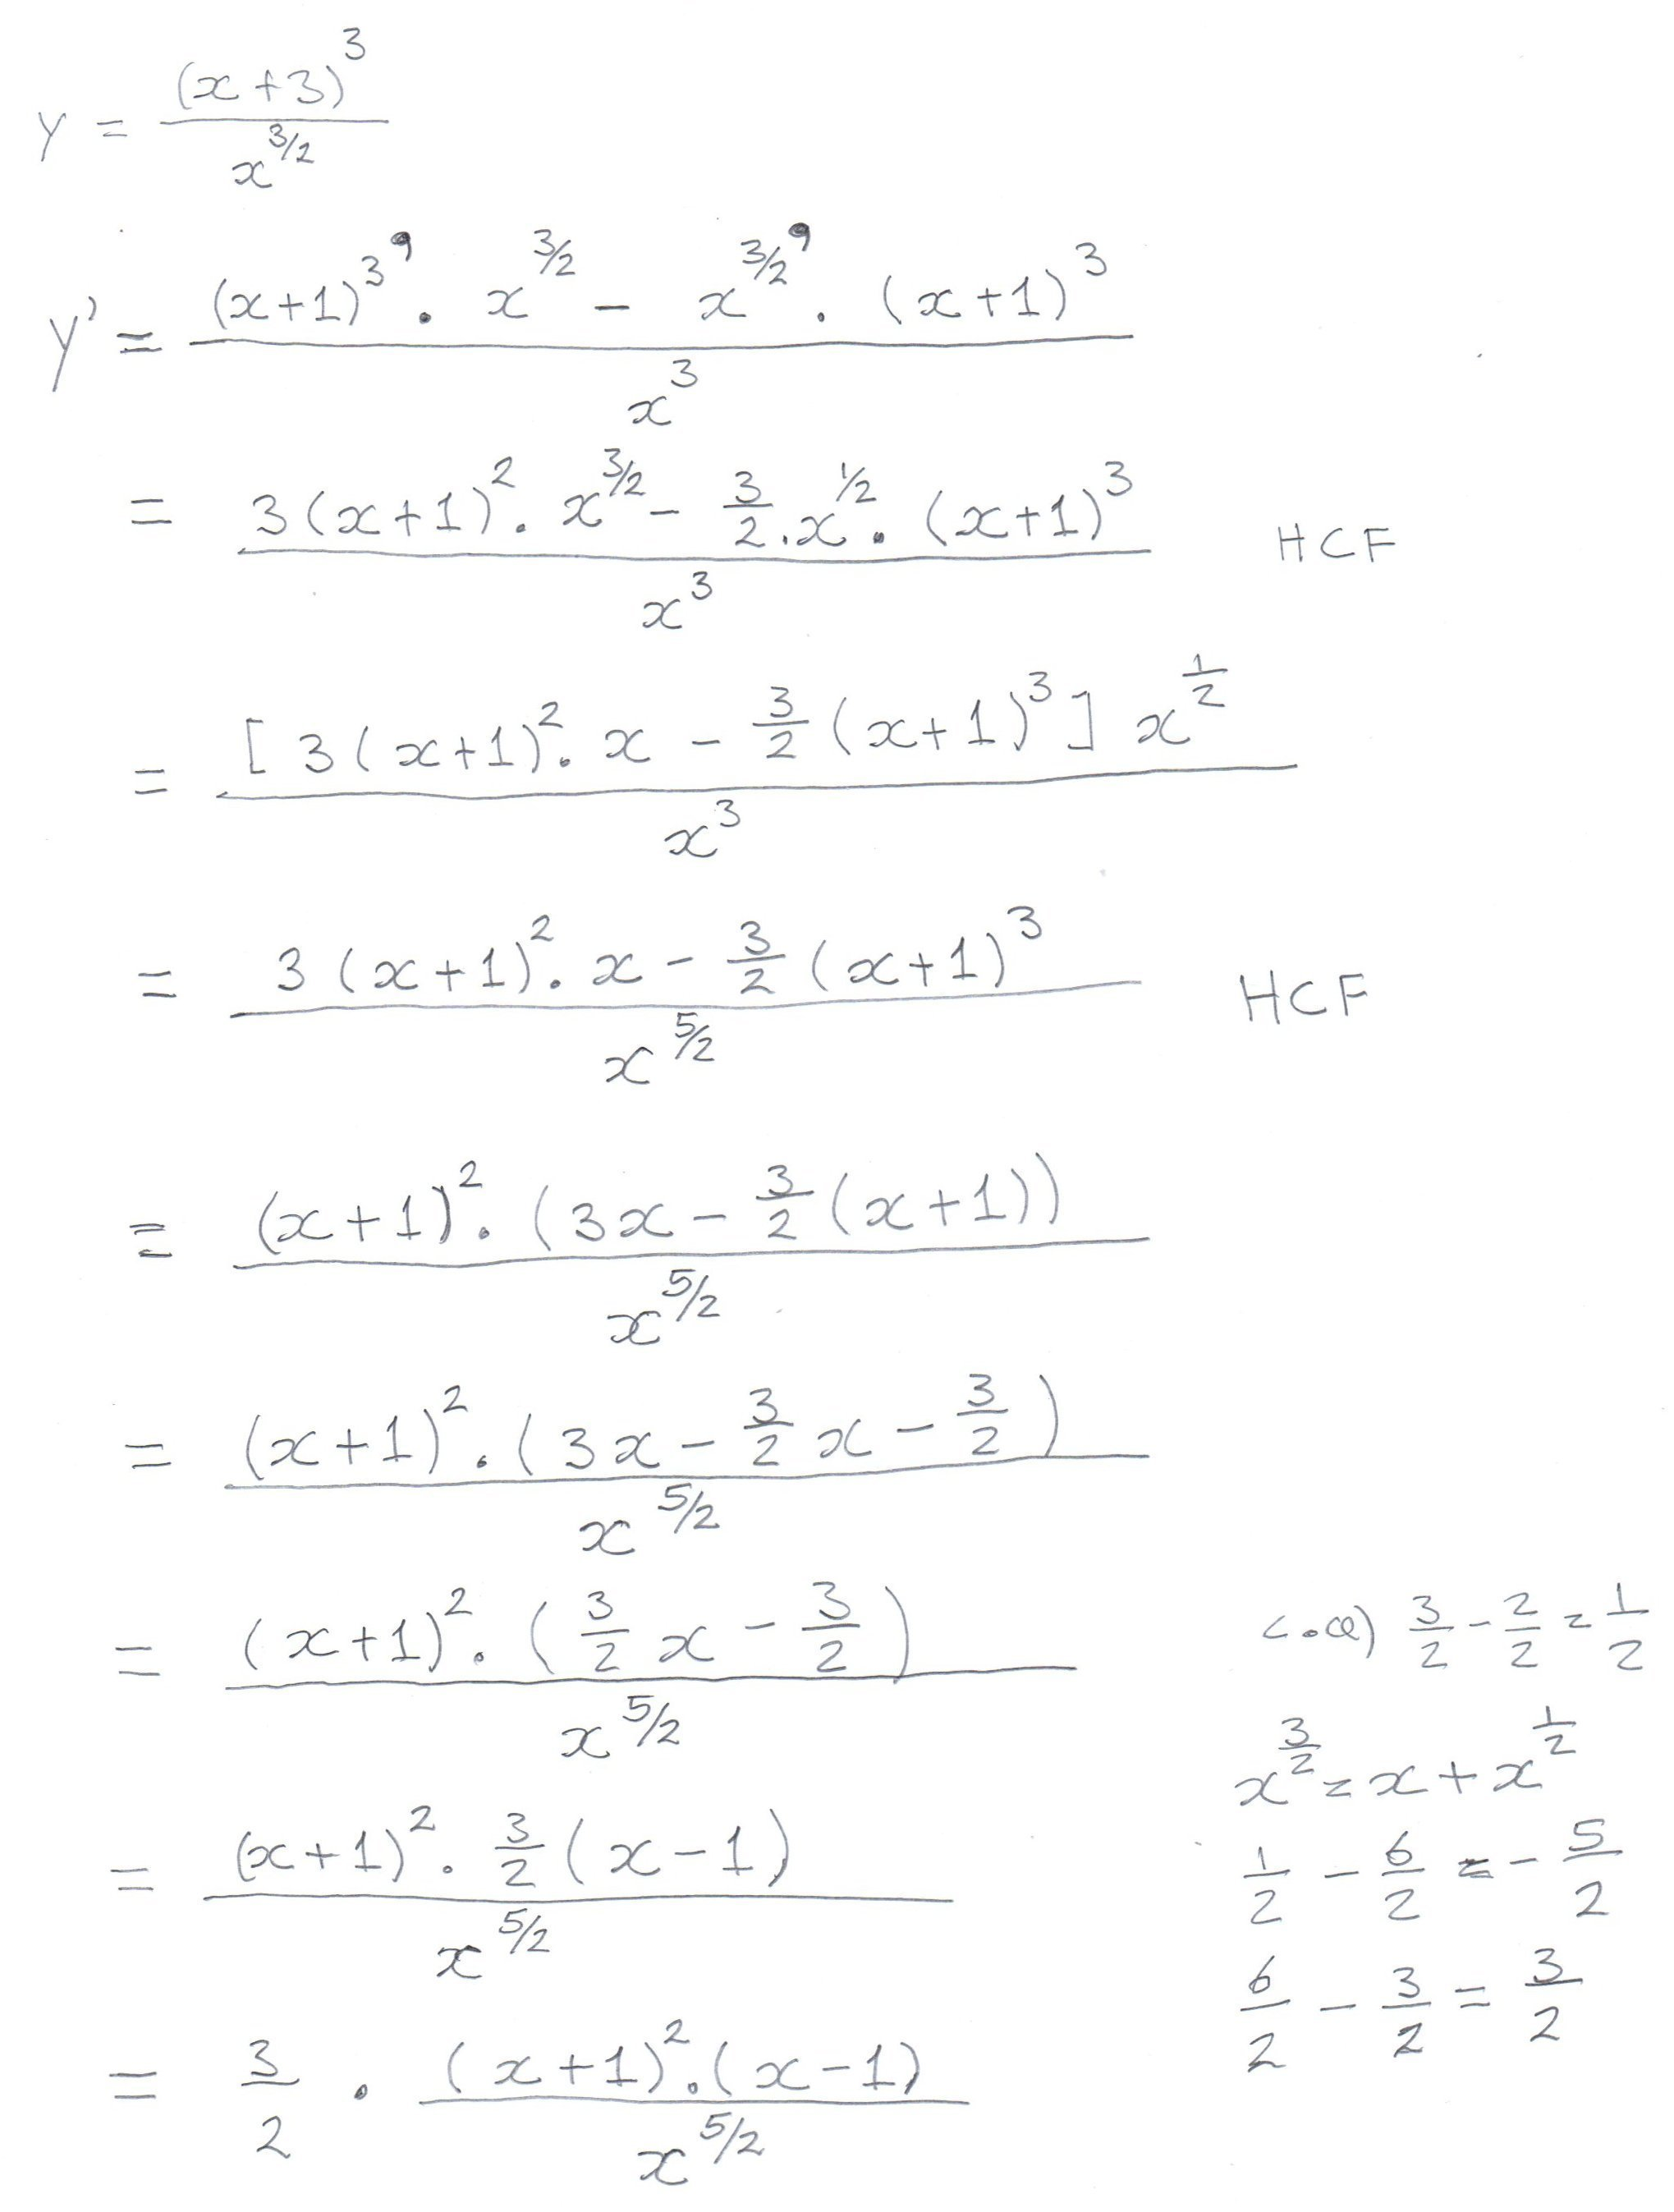
\includegraphics[scale=0.25]{./image/derivativeasy_2.jpg}
\end{minipage}
%%%%%%%%%%%%%%%%%%%%%%%%%%%%%%%%%%%%%%%%%%%%%%%%%%%%%%%%%%
%%%%%%%%%%%%%%%%%%%%%%%%%%%%%%%%
\newpage
\[\int x \; = \; \frac{x^2}{2}\]
\[\int_{-1}^{1}\sqrt{\frac{1+x}{1-x}}=\pi\]
\[e=\frac{1}{0!}+\frac{1}{1!}+\frac{1}{2!}+\frac{1}{3!}+...+\frac{1}{n!}+...\]
\newpage
%%%%%%%%%%%%%%%%%%%%%%%%%%%%%%%%%%%%%%%%%%%%%%%%%%%%%%%%%%%%%%%%%%%%%
 % Estudo da Cultura Organizacional segundo o Modelo Ogbonna & Harris
\section{Methods}
\acs{hcf} - highest common factor (pôr variável em evidência) 
\\
\\
\acl{factorisation} 
\\
\\
\acs{lcd-1} or \acs{lcm} - Lowest common denominator or lowest common multiple
%%%%%%%%%%%%%%%%%%%%%%%%%%%%%%%%%%%%%%%%%%%%%%%%%%%%%%%%%%%%%%%%%%%%%%%%%%%%%%%%%
 % Conclusões

%\todo[inline]{Always improve when possible !}
\bibliography{./bibliography/Bibliography}
\newpage
\appendix
\newpage
\footnote{Apontamento}
\end{document}
%%%%%%%%%%%%%%%%%%%%%%%%%%%%%%%%%%%%%%%%%%%%%%%%%%%%%%%%%%%%%%%%%%%%%%%%%%%%%%%%%
%\selectbiblanguage{portuguese}
%\setbtxfallbacklanguage{english}
%%%%%%%%%%%%%%%%%%%%%%%%%%%%%%%%%%%%%%%%%%%%%%%%%%%%%%%%%%%%%%%%%%%%%%%%%%%%%%%%%
%%%%%%%%%%%%%%%%%%%%%%%%%%%%%%%%%%%%%%%%%%%%%%%%%%%%%%%%%%%%%%%%%%%%%%%%%%%%%%%%%
\begin{comment}
Usando o método Socrático podemos perguntar qual a melhor ou melhores culturas organizacional que se enquadra na nacional nos vários tipos de organizações existentes.\\
%%%%%%%%%%%%%%%%%%%%%%%%%%%%
Para criar uma cultura na organização deve-se definir uma missão, valores, visão e os objetivos.\\
%%%%%%%%%%%%%%%%%%%%%%%%%%%%
Durante muito tempo tem havido estudos para descobrir a formula mágica que leva as organizações a ter sucesso, existe muitas abordagens com diferentes perspectivas, algumas convergem e outras divergem, e assim foram criados novos conceitos de forma a encapsular estilos e tipos de forma a poder se identificar quais são os mais propícios a ter uma maior elevada taxa de sucesso, conceitos tais como comportamento organizacional, cultura organizacional, performance organizacional, etc.\\
%%%%%%%%%%%%%%%%%%%%%%%%%%%%%
GENDER:
Nearly half of the U.S. workforce is now made up of women, and women are a growing percentage of the workforce in most countries throughout the world. Organizations need to ensure that hiring and employment policies create equal access and opportunities to individuals, regardless of gender.
RACE:
The percentage of Hispanics, blacks, and Asians in the U.S. workforce continues to increase. Organizations need to ensure that policies provide equal access and opportunities, regardless of race.
NATIONAL ORIGIN:
A growing percentage of U.S. workers are immigrants or come from homes where English is not the primary language spoken. Because employers in the United States have the right to demand that English be spoken at the workplace during job-related activities, communication problems can occur when employees’ English language skills are weak.
AGE:
The U.S. workforce is aging, and recent polls indicate that an increasing percentage of employees expect to work past the traditional retirement age of 65. Organizations cannot discriminate on the basis of age and need to make accommodations for the needs of older workers.
DISABILITY:
Organizations need to ensure that jobs and workplaces are accessible to the mentally, physically, and health challenged.
DOMESTIC PARTNERS
An increasing number of gay and lesbian employees, as well as employees with live-in partners of the opposite sex, are demanding the same rights and benefits for their partners that organizations have provided for traditional married couples.
RELIGION:
Organizations need to be sensitive to the customs, rituals, and holidays, as well as the appearance and attire, of individuals of non-Christian faiths such as Judaism, Islam, Hinduism, Buddhism, and Sikhism, and ensure that these individuals suffer no adverse impact as a result of their appearance or practices.
Tipos de descriminação:
sexual, intimidação, insultos e coerção, exclusão, incivilidade.
A satisfação melhora o desempenho.\\
%%%%%%%%%%%%%%%%%%%%%%%%%
Nas empresas publicas, o estimulo é sentido em menor grau ou não existente, consoante o tipo e características concretas da organização.\\
%%%%%%%%%%%%%%%%%%%%%%%%%
Nas organizações sem fim lucrativos e/ou dependentes do estado, existe outro tipo de estimulo os interesses dos governantes, quando o estado é parceiro ou responsável pela organização, os interesses de grupos de pressão da sociedade, etc.\\
%%%%%%%%%%%%%%%%%%%%%%%%%
Nas organizações sem fins lucrativos os objetivos estão em permanente discusão e/ou a ser alterados, resultando uma maior indefinição sobre as atividades a desenvolver por responsáveis e por colaboradores.\\
%%%%%%%%%%%%%%%%%%%%%%%%%
Teoria de Geer Hofteed.\\
%%%%%%%%%%%%%%%%%%%%%%%%%%
Best practices can come from national, say the American National Standards Institute (ANSI) or the Canadian Standards Association (CSA), or international, say ISO or Institute of Electrical and Electronics Engineers (IEEE), standards organizations, professional associa-tions, or consulting firms.\\
%%%%%%%%%%%%%%%%%%%%%%%%%
Eliminar desperdício e resolução de problemas.\\
%%%%%%%%%%%%%%%%%%%%%%%%%
Confiança na liderança e operadores.\\
%%%%%%%%%%%%%%%%%%%%%%%%%
Leaders have long been viewed as a primary influence on the creation of organizational culture (e.g. Bennis and Nanus, 1985; Schein, 1983). According to Schein (1985), the “only thing of real importance that leaders do is to create and manage culture”\\
%%%%%%%%%%%%%%%%%%%%%%%%%
Constante mudança de adaptação ao meio ambiente.\\
%%%%%%%%%%%%%%%%%%%%%%%%%
acknowledge that even in US and European companies, success rates are
not spectacular regarding efforts to change vision, values, and culture or business systems
and processes (Beer and Nohria, 2000; Beer et al., 1990; Carr et al., 1996).\\
%%%%%%%%%%%%%%%%%%%%%%%%%
Característica de bons Objetivos\\
- Claros\\
- Concisos\\
- Calendarizados\\
- Atingíveis\\
%%%%%%%%%%%%%%%%%%%%%%%%%
Tipos de organizações\\
- Organização privadas com fins lucrativos\\
- Organização privadas sem fins lucrativos\\
- Organização publicas com fins lucrativos\\
- Organização publicas sem fins lucrativos\\
%%%%%%%%%%%%%%%%%%%%%%%%%
tipos de hierarquias\\
tipos de departamentalizações\\
organização por processo\\
%%%%%%%%%%%%%%%%%%%%%%%%%
A divisão do trabalho, permitiu a redução do tempo de aprendizagem, isto é, cada um tem as suas funções, aumentando a produtividade. Cada um executa uma parte das tarefas necessárias a fabricação.\\
%%%%%%%%%%%%%%%%%%%%%%%%%
Gestão:
\emptyline
\begin{minipage}{20cm}
\begin{minipage}{5cm}
Instrumentos
\begin{enumerate}
\item Planear
\item Organizar
\item Controlar\\ \\
\end{enumerate}
\end{minipage}
\begin{minipage}{5cm}
Funções
\begin{enumerate}
\item Liderança
\item Comunicação
\item Motivação
\item Tomada de decisão
\end{enumerate}
\end{minipage}
\end{minipage}
%%%%%%%%%%%%%%%%%%%%%%%%%
Cadeia de valor\\
-Atividades principais\\
-Atividades de suporte\\
%%%%%%%%%%%%%%%%%%%%%%%%%
Cadeia de valor da organização é a sequencia de atividades e fluxos de informação que uma organização e os seus fornecedores devem desenvolver para desenhar, produzir, oferecer, entregar e suportar os seus produtos, estas são as atividades principais.\\
%%%%%%%%%%%%%%%%%%%%%%%%%
As atividades de suporte são as que apoiam um bom desempenho na realização das actividades principais.\\
- atividade administrativa e financeira\\
- atividade da gestão do pessoal\\
- atividade jurídica\\
- planeamento, controlo e gestão\\
- gestão de sistemas e tecnologia\\
%%%%%%%%%%%%%%%%%%%%%%%%%%
A atividade de suporte não contribuem diretamente para a criação do valor.\\
%%%%%%%%%%%%%%%%%%%%%%%%%%
Atividades de suporte e principal.\\
funções da Gestão sã Instrumental, Comportamental e Estrutural.\\
%%%%%%%%%%%%%%%%%%%%%%%%%%
Cumprir os objetivos é ser eficaz.\\
%%%%%%%%%%%%%%%%%%%%%%%%%%%
Para gerir a produção (planear, organizar, dirigir e controlar), há que recolher um elevado volume de informação de controlo, sendo frequentemente necessário refazer o planeamento.\\
%%%%%%%%%%%%%%%%%%%%%%%%%%%
- Implementação por projeto\\
- Implementação por processo\\
- Implementação por células\\
- Implementação por cadeia ou em linha\\
- Implementação por produto\\
%%%%%%%%%%%%%%%%%%%%%%%%%%
Na implementação por célula de fabrico procura agrupar os produtos segundo a semelhança das suas rotinas operatórias.\\
Na implementação por processo, é possível cada serie (ou lote) ser processado integralmente num dado centro, antes de avançar para o centro onde irá sofrer a operação de transformação seguinte.\\
A análise ABC pode ser utilizada para averiguar quais as principais encomendas responsáveis pela sobrecarga de um dado centro de trabalho.\\
%%%%%%%%%%%%%%%%%%%%%%%%%%
Organizar é estipular quem faz o quê, atribui-se os recursos necessários para o fazer, criar um sistema de informação para verificar execução.\\
%%%%%%%%%%%%%%%%%%%%%%%%%%%
O que lhes chama a atenção e medem; suas reações a incidentes criticos, alocação de meios, papeis assumidos, e partilha de informação; recompensas e delegação de poder; recrutamento, seleção e promoção. As lideranças chave tem como responsabilidade de modificar a cultura de forma a estar atualizada com as mudanças exigidas.\\
%%%%%%%%%%%%%%%%%%%%%%%%%%%%
Aqui distingue-se dois tipos de lideres os transacionais e os de transformação. “culture affects leadership  as much as leadership affects culture”
%%%%%%%%%%%%%%%%%%%%%%%%%%%%
Planear é estabelecer os objetivos a atingir e o percurso de ações.\\
%%%%%%%%%%%%%%%%%%%%%%%%%%%%
A formulação, avaliação e seleção de estratégias e o desenvolvimento dos planos mais detalhados para as pôr em prática são feitos após a definição da missão e da análise do meio ambiente da organização.\\
%%%%%%%%%%%%%%%%%%%%%%%%%%%%
Ferramentas para avaliar o cumprimento dos objetivos\\
- benchmarking\\
- scorecard management\\
- Banco de Portugal\\
%%%%%%%%%%%%%%%%%%%%%%%%%%%%
Método de demonstrar o desempenho de uma organizações através da eficacia, eficiência e seu rendimento.\\
%%%%%%%%%%%%%%%%%%%%%%%%%%%%%
Eficacia avalia em que medida os objetivos estão alinhados com a necessidades sociais que ela se propõe a satisfazer, ou seja, em que medida os seus objetivos são a tal adequados.\\
%%%%%%%%%%%%%%%%%%%%%%%%%%%%%
Eficiência avalia a economia de recursos utilizados para realizar os seus objetivos, requer uma boa estruturação dos processos seguidos nas atividades, o que leva tempo e custa dinheiro.\\
%%%%%%%%%%%%%%%%%%%%%%%%%%%%%
Missão - SWOT Meio Ambiente (transacional e contextual(PEST)) - Objetivos - Implementação.\\
%%%%%%%%%%%%%%%%%%%%%%%%%%%%%
O sucesso das empresas está correlacionada positivamente com o seu planeamento.\\
%%%%%%%%%%%%%%%%%%%%%%%%%%%%%
Na análise do meio ambiente transacional, analisa-se o comportamento previsional das entidades com quem a organização interage.\\
%%%%%%%%%%%%%%%%%%%%%%%%%%%%%
Controlo.\\
O controlo pode ser encarado como um processo de aprendizagem.\\
O controlo deve servir, acima de tudo, para ajudar a garantir que os objetivos estabelecidos são atingidos.\\
Se a informação recolhida e os resultados apurados no processo de controlo não conduzem a ações de correção quando necessário, este será não só inútil, mas até prejudicial.\\
O recurso aos sistemas de informação permite, em geral, simplificar os procedimentos de controlo.\\
%%%%%%%%%%%%%%%%%%%%%%%%%%%%%%%
Controlar é os procedimentos de verificar sua execução, estar atento a imprevistos e pronto a correções recorrendo a re-organização e/ou novo planeamento, também pode-se optar por não fazer nada.\\
%%%%%%%%%%%%%%%%%%%%%%%%%%%%%%%%
Estilos de liderança:
\begin{itemize}
\item participative leadership\\
Is gauged by the extent to which leaders allow subordinates to influence decisions by requesting input and contribution.
\item supportive leadership\\
Focuses on the degree to which the behaviour of a leader can be viewed as sympathetic, amicable, and considerate of subordinate needs.
\item Instrumetal leadership\\
This measure of leadership style is akin to directive or transactional leadership and is designed to measure the extent to which leaders specify expectations, establish procedures, and allocate tasks.
\end{itemize}
Motivação teorias Moslow, Hersberg, Victor Vroom.\\
Se as condições e recompensas oferecidas aos funcionários não lhes permitirem satisfazerem algumas das suas necessidades, mais facilmente abandonam a equipa ou organização a que pertencem.\\
Motivação é o conjunto de fatores que provocam, canalizam e sustentam o comportamento das pessoas.\\
Um gestor interessado em atingir um bom desempenho estabelece objetivos atingíveis e bem defendidos.\\
Auto-confiança no desenvolvimento do trabalho pode diminuir a sua motivação.\\
Motivar é criar condições necessárias para que as pessoas se empenham na prossecução dos objetivos da organização.\\
O impacto da comunicação no desempenho da organização é muito elevado.\\
Os Gestores tem de ser coerentes e alinhados com o que transmitem de forma a criar uma estrutura de confiança.\\
Um líder de uma organização é aquele que detém capacidades de influenciar os colaboradores.\\
gestão das atividades é o exercício do poder de um gestor.\\
poder de premiar e punir é suficiente para gerir as atividades do dia a dia.\\
poder informacional.\\
Um sistema de avaliação do desempenho de uma empresa é uma valia porque é uma boa oportunidade para analisar o grau de cumprimento dos objetivos acordados.\\
A medida que as organizações se achatam, os gestores têm de aprender a permitir que os seus colaboradores tomem decisões e tenham informação sobre questões mais sensíveis.\\
Para um engenheiro é muito útil conhecer os aspectos essenciais da legislação laboral.\\
A gestão das pessoas é cada vez mais importante porque são as pessoas que têm o conhecimento e só as pessoas o podem partilhar e aplicar.\\
Numa organização, apoiar e compensar as pessoas é fundamental, mas também é indispensável falar com elas sobre os erros que cometem no sentido de serem corrigidas e evitadas no futuro.\\
Uma organização tem maior probabilidade de ter sucesso se gerir as pessoas de modo a que estas ao contribuírem para o sucesso da organização tenham também sucesso elas próprias.\\
A qualidade é a totalidade das características de um produto ou serviço, que determinam a sua aptidão para satisfazer determinadas necessidades.\\
Garantia da qualidade tem como objetivo primeiro, o controlo do processo, ou seja, a minimização ou mesmo eliminação dos erros na produção.\\
A garantia da qualidade concentra-se no controlo do processo produtivo e controlo do produto.\\
Os custos relacionados com a insatisfação dos clientes são considerados custos de não qualidade.\\
O diagrama de Pareto permite identificar rapidamente as causas vitais e as triviais de um dado problema.\\
As cartas de controlo destinam-se a detetar as variações resultantes da alteração, frequentemente de natureza aleatória e acidental, de algum dos parâmetros de processo de fabrico (ditas causas especiais).\\
As sete ferramentas clássicas da qualidade\\
- Fluxograma\\
- Registo e análise de dados\\
- Diagrama de causa - efeito (espinha de peixe 4M)\\
- Diagrama de Pareto\\
- Histogramas\\
- Diagramas de dispersão\\
- Cartas de Controlo\\
tipos de lideres\\
- Autocrático\\
- Participativo \\
- Democrático \\
- Deixa andar\\
estilo de líder\\
- Orientado as pessoas\\
- Orientado as tarefas\\
%%%%%%%%%%%%%%%%%%%%%%%%%%%
The relationship between culture and leadership appears to be reciprocal—top leaders create and maintain an organizational culture, which in turn influences the values, attitudes, and behaviors of middle and entry-level leaders. Although leader–culture fit has not been specifically studied in the published literature, we believe that there is value in examining the match between a leader’s behaviors and the culture in which they work. While research hasn’t examined this at the level we discuss, current research does suggest that fit is important at the national level and at the leader–follower level. Expansion of this research will help determine what aspects of leader culture fit are determinants of leader and organizational effectiveness. Although there are a variety of approaches that researchers can take to examining leader–culture fit, we offer the following recommendations. First, although studies of perceived fit are of limited value, the ease of collecting this data should motivate researchers to start thinking about adding questions concerning leader–culture fit. Given the lack of published findings, this research can begin shaping our knowledge about this phenomenon. Second, while studies of subjective fit will be more important, researchers should utilize 360-degree measurement systems in order to also obtain the most objective fit indices possible. This practice will likely tell us more about the impact of fit than just examining leaders’ self-reports. Third, it is important to measure culture at the aggregate level in order to ensure that the actual values of the organization are being captured, not just the leader’s values. Although these recommendations may be difficult to achieve in practice, they offer the best hope of leveraging leader–culture fit for the future.\\
%%%%%%%%%%%%%%%%%%%%%%%%%%%%%%%%%
A atividade comportamental consiste em lidar com pessoas, comunicar instruções e receber feedback, propiciar a comunicação entre os terceiros, motivar, tomar decisões e criar condições para que os colaboradores também o possam fazer, assegurar a liderança para cumprir a execução.\\
%%%%%%%%%%%%%%%%%%%%%%%%%%%%%%%%%%
More specifically, it suggests that culture provides the normative bounds for transactional leaders to be effective and that transformational leaders influence culture through strategic decisions and vision, by celebrating success, and by identifying and rewarding employees. \\
%%%%%%%%%%%%%%%%%%%%%%%%%%%%%%%%%%
In sum, leadership and organizational culture are related, and further, the dynamics between these constructs impact organizational effectiveness. However, the theoretical work in this area largely outweighs the empirical, and we believe there is utility in adopting a “fit” perspective for further research in this area.\\
%%%%%%%%%%%%%%%%%%%%%%%%%%%%%%%%%%
In their meta-analysis, Kristof-Brown et al. (2005) identified five types of fit research that captured the majority of published studies: person–vocation fit, person–job fit, person–organization fit, person–group fit, and person–supervisor fit. Attempting to integrate all of these perceptions of fit, Jansen \& Kristof-Brown (2006) proposed a multidimensional theory of person–environment (PE) fit.\\
%%%%%%%%%%%%%%%%%%%%%%%%%%%%%%%%%%%
O alinhamento entre o líder e a cultura da organização influencia a sua eficacia.\\
%%%%%%%%%%%%%%%%%%%%%%%%%%%%%%%%%%%
A vida ensina e se não aprendemos ela insiste e persiste até morrermos.\\
A liberdade é medida pela quantidade de ética e moralidade presente na sociedade.\\
Respect is always earned never a given.\\
\end{comment}
%%%%%%%%%%%%%%%%%%%%%%%%%%%%%%%%%%%%%%%%%%%%%%%%%%%%%%%%%%%%%%%%%%%%%
%%%%%%%%%%%%%%%%%%%%%%%%%%%%%%%%%%%%%%%%%%%%%%%%%%%%%%%%%%%%%%%%%%%%%
